% !TEX TS-program = pdflatexmk
% !TEX root = EUDAQUserManual.tex
\documentclass[12pt, oneside, notitlepage, a4paper]{scrartcl}
\usepackage{epsfig, scrpage2, graphicx, listings, microtype, setspace, upquote}
\usepackage[british]{babel}
\usepackage{hyperref} % must be the last package (apart from glossaries)
\usepackage[toc, nonumberlist]{glossaries} % must go after hyperref, so entries are clickable

\setcounter{secnumdepth}{3}
\setcounter{tocdepth}{2}

\setlength{\parindent}{0em}
\setlength{\parskip}{0ex plus0.5ex minus0ex}
\pagestyle{scrheadings}

\def\subsectionautorefname{section}
\def\subsubsectionautorefname{section}
%\let\stdsection\section
%\renewcommand\section{\newpage\stdsection}

% Some useful commands
\newcommand*\micron{\ensuremath{\mu\mathrm{m}}}
\newcommand*\micro{\ensuremath{\mu}}
\newcommand*\square{\ensuremath{^2}}
\newcommand*\degree{\ensuremath{^\circ}}
\newcommand*\lt{\ensuremath{<}}
\newcommand*\gt{\ensuremath{>}}
\newcommand*\x{\ensuremath{\times}}
\newcommand*\param[1]{\ensuremath{\langle}#1\ensuremath{\rangle}}

\newcommand*\ttitem[1]{\item[\texttt{#1}\,:]}
\newcommand*\ccitem[1]{\item[]\lstinline[style=shaded,language=C++]{#1}}
%\lstMakeShortInline[style=plain,language=C++]@
\newcommand*\inline[2][C++]{\lstinline[style=plain,language=#1]{#2}}
\newcommand*\myinputlisting[3][C++]{
Latest version available at:\\
\textls[#2]{\url{https://github.com/eudaq/eudaq/blob/master/#3}}

\lstinputlisting[style=full, language=#1]{../../#3}
\rule[\baselineskip]{\textwidth}{1pt}
}
\lstnewenvironment{listing}[1][C++]{\lstset{style=shaded,language=#1}}{}

\newenvironment{myitemize}
{\begin{itemize}%
  \setlength{\itemsep}{0.1\baselineskip}%
  \setlength{\parskip}{0pt}%
  \setlength{\parsep}{0pt}}
{\end{itemize}}
\newenvironment{mydescription}
{\begin{description}%
  \setlength{\itemsep}{0.1\baselineskip}%
  \setlength{\parskip}{0pt}%
  \setlength{\parsep}{0pt}}
{\end{description}}

\renewcommand*\headfont{\normalfont}

\renewcommand*\glsgroupskip{}
\renewcommand*{\glspostdescription}{.\vspace{-0.5\baselineskip}}
\makeglossaries

%\glsdisablehyper
%\defglsdisplay{\cooltooltip[1,1,0.9][1,1,1]{Glossary}{a #2}{}{b #2}{#1}}
%\renewcommand{\glsdisplay}[4]{%
%   \cooltooltip[1,1,1][1,1,0.9]{Definition}{#2}{}{#2}{#1#4}%
%} 

\lstset{
    %basicstyle=\ttfamily
    keywordstyle=\color[rgb]{0,0,0.8},
    %identifierstyle=\color[rgb]{0,0,0},
    commentstyle=\color[rgb]{0,0.4,0},
    stringstyle=\color[rgb]{0.4,0,0.8},
    showstringspaces=false,
    basewidth=1.2ex,
    numberstyle=\footnotesize\color[rgb]{0.6,0.6,0.6},
    stepnumber=1,
    numbersep=10pt,
    tabsize=2,
    breaklines=true,
    prebreak = \raisebox{0ex}[0ex][0ex]{\color[rgb]{0.6,0.6,0.6}\ensuremath{\hookleftarrow}},
    breakatwhitespace=true,
    %aboveskip={1.5\baselineskip},
    columns=fixed,
    upquote=true,
    extendedchars=false,
    framerule=0pt,
    belowskip={0.5\baselineskip},
}
\lstdefinestyle{plain}{
    basicstyle=\normalsize\ttfamily,
    numbers=none,
    frame=none,
    %belowskip={0.5\baselineskip},
    backgroundcolor={},
}
\lstdefinestyle{shaded}{
    basicstyle=\small\ttfamily,
    numbers=none,
    frame=single,
    backgroundcolor=\color[rgb]{1,0.98,0.95},
}
\lstdefinestyle{full}{
    basicstyle=\small\ttfamily,
    numbers=left,
    frame=single,
    %belowskip={\baselineskip},
    backgroundcolor=\color[rgb]{1,1,0.95},
}
\lstdefinelanguage{conf}{
    otherkeywords={=},
    alsoletter={[},
    alsoletter={]},
    moredelim=[s][keywordstyle]{[}{]},
    comment=[l]{\#},
    %morecomment=[l]{\;},
    %string=[s]',
    %morestring=[s]",
}
\lstdefinelanguage{mybash}[]{bash}{
    deletekeywords={test,read},
    morekeywords={svn,make,chown,chmod},
    %keywordsprefix={./},
    moredelim=[is][keywordstyle]{$[}{]$},
}


% Insert EUDET document number here:
\newcommand*\EUDETnum{EUDAQ User Manual}

% PDF info and link colours
\hypersetup{
  pdftitle={EUDAQ Software User Manual},
  pdfauthor={EUDAQ Development Team},
  pdfsubject={EUDET},
  pdfkeywords={EUDET, EUDAQ, Software, User Manual},
  colorlinks=true,
  linkcolor=black, % \ref \autoref \pageref
  citecolor=blue, % \cite
  urlcolor=blue, % \url \href (external)
  filecolor=blue, % \href (local file)
}

% Load glossary
\loadglsentries{src/glossary.tex}

% Headers and Footers
\titlehead{\EUDETnum}
\lehead{\EUDETnum}
\lohead{\EUDETnum}
\automark{section}
\rehead{\headmark}
\rohead{\headmark}
\chead{}
\cfoot{\pagemark}

% Title info
\subject{
\includegraphics[width=0.2\textwidth]{src/images/logo_eudet} 
\includegraphics[width=0.6\textwidth]{src/images/AIDA_logo_medium}}
\title{\Large EUDAQ Software User Manual} 
\author{\normalsize EUDAQ Development Team}
%%% THIS IS JUST A DUMMY FILE: CMake will generate the correct one when building the manual
\gdef\CMakeLibVersion{non-identified (not built with CMake)}
 % defines the \CMakeLibVersion command which is
                    % set by CMake to the current EUDAQ version number
                    % (with git hash tag)
\date{\normalsize As of \today \\ for EUDAQ version \CMakeLibVersion}

\begin{document}

% Title page
\maketitle
\begin{abstract}
\noindent
This document provides an overview of the EUDAQ software,
the data acquisition framework used by the EUDET JRA1 beam telescope.
It describes how to install and run the DAQ system and use many of the included utility programs,
and how users may integrate their systems into the EUDAQ framework
by writing their own Producer and DataConverterPlugin,
thus allowing them to take advantage of the EUTelescope analysis framework.
\end{abstract}
\newpage

% Contents
% Condense slightly to fit on one page
\begin{spacing}{0.92}
\tableofcontents
\end{spacing}

% Main sections
% !TEX root = EUDAQUserManual.tex
\section{Introduction}
The EUDAQ software is a data acquisition framework, written in C++,
and designed to be modular and portable, running on Linux, Mac OS X, and Windows.
It was written primarily to run the EUDET-type beam telescope~\cite{Roloff:2009zza,Jansen:2016},
but is designed to be generally useful for other systems.

The hardware-specific parts are kept separate from the core,
so that the core library can still be used independently.
For example, hardware-specific parts are two components for the EUDET-type beam telescope: \gls{TLU} and \gls{NI} for Mimosa 26 sensor read out.

The raw data files generated by the DAQ can be converted to the \gls{LCIO} format,
allowing for analysing the data using the EUTelescope package \cite{eutel2008}.

\subsection{Architecture}
It is split into a number of different processes,
each communicating using TCP/IP sockets (compare \autoref{fig:DAQ}).
A central Run Control provides an interface for controlling the whole DAQ system;
other processes connect to the Run Control to receive commands and to report their status.

\begin{figure}[htb]
  \begin{center}
    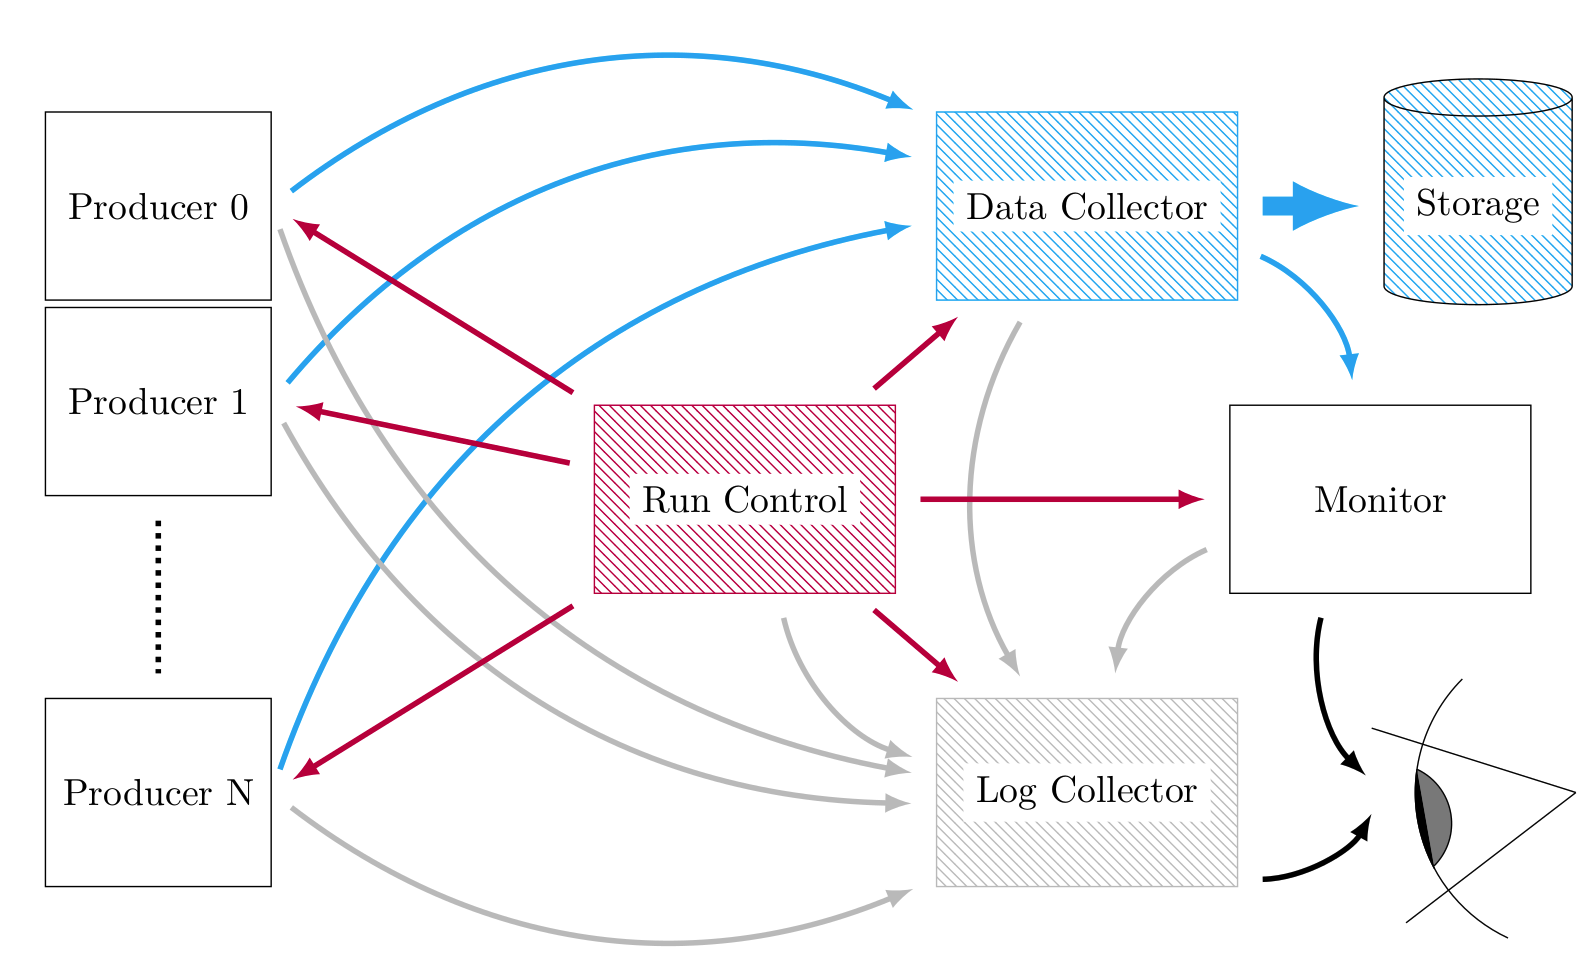
\includegraphics[width=0.9\textwidth]{src/images/eudaq_working_principle}
    \caption{Schematic of the EUDAQ architecture \cite{Spannagel:2016}.}
    \label{fig:DAQ}
  \end{center}
\end{figure}

Each hardware that produces data (e.g. the \gls{TLU}, the \gls{NI}, or a \gls{DUT}) will have a Producer process (on the left in \autoref{fig:DAQ}).
This will initialize, configure, stop and start the hardware by receiving the commands from the Run Control (red arrows), read out the data and send it to the Data Collector (blue arrows).

The Data Collector receives all the data streams from all the Producers,
and combines them into a single stream that is written to disk (Storage).
It writes the data in a native raw binary format,
but it can be configured to write in other formats, such as \gls{LCIO}.

The Log Collector receives log messages from all other processes (grey arrows),
and displays them to the user, as well as writing them all to file.
This allows for easier debugging, since all log messages are stored together in a central location.

The Monitor reads the data file and generates online-monitoring plots for display.
In the schematic it is shown to communicate with the Data Collector via a socket,
but it actually just reads the data file from disk.

\subsection{Directory and File Structure}
The EUDAQ software is split into several parts that can each be compiled independently,
and are kept in separate subdirectories.
The general structure is outlined below:

\begin{myitemize}
\item \texttt{main}
  contains the core EUDAQ library with the parts that are common to most of the software,
  and several command-line programs that depend only on this library.
  All definitions in the library should be inside the \texttt{eudaq} namespace.
  It is organised into the following subdirectories:
  \begin{myitemize}
  \item \texttt{lib/src}
    contains the library source code,
  \item \texttt{exe/src}
    contains the (command line) executables source code,
  \item \texttt{include}
    contains the header files inside the \texttt{eudaq} subdirectory (to match the namespace),
  \end{myitemize}
\item \texttt{gui}
  contains the graphical programs that are built with Qt, such as the RunControl and LogCollector.
\item \texttt{producers}
  contains all (user-provided) producers shipped with the EUDAQ
  distribution, for example:
  \begin{myitemize}
\item \texttt{tlu}
  contain the parts that depend on the \gls{TLU}.
\item \texttt{ni}
  contain the parts that depend on the \gls{NI} system for Mimosa 26 read out.
\item e.g. \texttt{depfet}, \texttt{fortis}, \texttt{taki}\ldots{}
  contain the code for third-party producers that have been used with
  EUDET-type beam telescopes.
  \end{myitemize}
\item \texttt{extern}
  stores external software that is not part of EUDAQ itself, but that is needed by EUDAQ in some cases,
  such as the \texttt{ZestSC1} driver and the \texttt{tlufirmware} for the \gls{TLU}.
% and the Tsi148 VME driver.
\item \texttt{bin} and \texttt{lib}
  contain the compiled binaries (executables and libraries) generated from the other directories.
\item \texttt{conf}
  contains configuration files for running the beam telescope.
\item \texttt{data} and \texttt{logs}
  are directories for storing the data and log files generated while running the DAQ.
\item \texttt{doc}
  contains documentation, such as this manual.
\end{myitemize}

Each directory containing code has its own \texttt{src} and \texttt{include} subdirectories,
as well as a local \texttt{CMakeLists.txt} file containing the rules
for building that directory using \texttt{CMake}.
Header files usually have a \texttt{.hh} extension so that they can be automatically recognised as C++
(as opposed to C), and source files have either \texttt{.cc} for parts of a library or \texttt{.cxx} for executables.

Each directory can contain a \texttt{README.md} file for brief documentation for this specific part, e.g.  
as installation advice. 
Using the \texttt{*.md} file ending allows for applying the Markdown language \cite{markdownWWW}. 
Accordingly, content will be formatted on the the GitHub platform, where the code is hosted online.

% !TEX root = EUDAQUserManual.tex
\section{Installing EUDAQ}

The installation is described in four steps:%
\footnote{A quick installation manual is also described in the \texttt{README.md}, e.g. \url{https://github.com/eudaq/eudaq/blob/v1.6-dev/README.md}.}
\begin{enumerate}
\item Installation of (required) prerequisites
\item Downloading the source code (GitHub)
\item Configuration of the code (CMake)
\item Compilation of the code
\end{enumerate}

If you occur problems during the installation process, please have a look into the issue tracker on GitHub.%
\footnote{Go to \url{https://github.com/eudaq/eudaq/issues}} 
Here you can search, if your problem had already been experienced by someone else, or you can open a new issue (see \autoref{sec:reporting}).

\subsection{Installation of prerequisites}

EUDAQ has few dependencies on other software, but some features do rely on other packages:
\begin{itemize}
\item To get the code and stay updated with the central repository on GitHub git is used.
\item To configure the EUDAQ build process, the CMake cross-platform, open-source build system is used.
\item To compile EUDAQ from source code requires a compiler that implements the C++11 standard.
\item The libusb library is needed to communicate over USB with a \gls{TLU} \cite{Cussans2009}.
\item Qt is required to build GUIs of the e.g. Run Control Log Collector. 
\item ROOT is required for the Online Monitor.
\end{itemize}

\subsubsection{Git}
Git is a free and open source distributed version control and is available for all of the usual platforms \cite{gitWWW}. 
It allows for local version control and repositories, but also communicating with central online repositories like GitHub.
   
In order to get the EUDAQ code and stay updated with the central repository on GitHub git is used (see \autoref{sec:downloadingEUDAQ}).
But also for developing the EUDAQ code having different versions (tags) or branches (development repositories), git is used (see \autoref{sec:contributing}).


\subsubsection{CMake (required)}
In order to automatically generate configuration files for the build process of EUDAQ both compiler and platform independent, the CMake build system is used.

CMake is available for all major operating systems from \url{http://www.cmake.org/cmake/resources/software.html}. On most Linux distributions, it can usually be installed via the built-in package manager (aptitude/apt-get/yum etc.) and on OSX using packages provided by e.g. the MacPorts or Fink projects.

\subsubsection{C++11 compliant compiler (required)}
The compilation of the EUDAQ source code requires a C++11 complianti compiler and has been tested with GCC (at least version 4.8), Clang (at least version 3.1), and MSVC (Visual Studio 2012 and later) on Linux, OS X and Windows.

If you are using Scientific Linux, please install the \emph{Developer Toolset} available e.g. from \url{http://linux.web.cern.ch/linux/devtoolset/} to get access to a GCC version which fully implements C++11, e.g. on SL6 do
\begin{listing}[mybash]
scl use devtoolset-1.1 bash
\end{listing}
and cmake and install in this bash.

\subsubsection{libusb (for the EUDET TLU)}
In order to communicate over USB with a \gls{TLU}, the libusb library is needed.
Therefore, if you want to compile the \texttt{tlu} subdirectory, you should make sure that libusb is properly installed.

On Mac OS X, this can be installed using Fink or MacPorts.
If using MacPorts you may also need to install the \texttt{libusb-compat} package.

On Linux it may already be installed,
otherwise you should use the built-in package manager to install it.
Make sure to get the development version, which may be named \texttt{libusb-devel} instead of simply \texttt{libusb}, e.g. on Ubuntu: 
\begin{listing}[mybash]
sudo apt-get install libusb-dev 
\end{listing}

On Windows, libusb is only needed if compiling with cygwin,
in which case you should use the cygwin installer to install libusb.
Otherwise libusb is not needed, as the included ZestSC1 libraries should work as they are.

\subsubsection{ZestSC1 drivers and TLU firmware files (for the EUDET TLU)}
Additonally to the libusb library, the EUDET \gls{TLU} producer requires the
ZestSC1 driver package and the FPGA firmware bitfiles. 
These are available to download via AFS from DESY. 
If AFS is accessible on the machine when CMake is run, the necessary files will be installed
automatically.
Otherwise, manually copy full folder with sub-directories from
\begin{itemize}
\item \texttt{/afs/desy.de/group/telescopes/tlu/ZestSC1} and
\item \texttt{/afs/desy.de/group/telescopes/tlu/tlufirmware}
\end{itemize}
into the \texttt{extern} subfolder in your EUDAQ source directory.


\subsubsection{Qt (for GUIs)}
The graphical interface of EUDAQ uses the Qt graphical framework.
In order to compile the \texttt{gui} subdirectory, you must therefore have Qt installed.
It is available in most Linux distributions as the package \texttt{qt4-devel} or  \texttt{qt5-devel}
but make sure the version is at least 4.4, since there are a few issues with earlier versions.

If the included version is too old, or on other platforms,
it can be downloaded from \url{http://qt.nokia.com/downloads}.
Select the LGPL (free) version, then choose the complete development environment
(it may also work with just the framework, but this is untested).
Make sure the \texttt{QTDIR} environment variable is set to the Qt installation directory,
and the \texttt{\$QTDIR/bin} directory is in your path.

If you are using OSX, the easiest way to install Qt is using the
packages provided by the MacPorts project (\url{http://www.macports.org/}).

\subsubsection{ROOT (for Monitor)}
\label{sec:Root}
The Online Monitor, as well as a few command-line utilities (contained in the \texttt{root} subdirectory), use the ROOT package for histogramming.
It can be downloaded from \url{http://root.cern.ch} or installed via
your favorite package manager.

Make sure ROOt's \texttt{bin} subdirectory is in your path, so that the \texttt{root-config} utility can be run.
This can be done by sourcing the \texttt{thisroot.sh} (or \texttt{thisroot.ch} for csh-like shells)
script in the \texttt{bin} directory of the ROOT installation:
\begin{listing}[mybash]
source /path-to/root/bin/thisroot.sh
\end{listing}

\subsubsection{LCIO / EUTelescope (for converting/analysis)}
\label{sec:LCIO-EUTel}
To enable the writing of \gls{LCIO} files, or the conversion of native files to \gls{LCIO} format,
EUDAQ must be linked against the \gls{LCIO} and EUTelescope libraries.
Detailed instructions on how to install both using the
\texttt{ilcinstall} scripts can be found at \url{http://eutelescope.web.cern.ch/content/installation}.

The \texttt{EUTELESCOPE} and \texttt{LCIO} environment variables should be set to the
installation directories of EUTelescope and LCIO respectively.
This can be done by sourcing the \texttt{build\_env.sh} script as follows:
\begin{listing}[mybash]
source /path-to/Eutelescope/build_env.sh
\end{listing}

%%%%%%%%%%%%%%%%%%%%%%%%%%%%%%%%%%%%%%%%%%%%%%%%%%%%%%%%%%%
\subsection{Download the source code from GitHub}
\label{sec:downloadingEUDAQ}

The EUDAQ source code is hosted on GitHub \cite{githubEUDAQ}. 
Here, we describe how to get the code and install a stable version release. 
In order to get information about the work flow of developing the EUDAQ code, please find the relevant information in see \autoref{sec:contributing}.

\subsubsection{Downloading the code (clone)}
We recommend to obtain the software by using git,
since this will allow you to easily update to newer versions.
The source code can be downloaded with the following command:
\begin{listing}[mybash]
git clone https://github.com/eudaq/eudaq.git eudaq
\end{listing}
This will create the directory \texttt{eudaq}, and download the latest
version into it. 

\textit{Note:} Alternatively and without version control, you can also download a zip/tar.gz file of EUDAQ releases (tags) from \url{https://github.com/eudaq/eudaq/releases}. 
By downloading the code, you can skip the next two subsections. 

\subsubsection{Changing to a release version (checkout)}
After cloning the code from GitHub, your local EUDAQ version is on the master branch (check with \texttt{git status}).  
For using EUDAQ without development or for production environments (e.g. at test beams), we strongly recommend to use the latest release version. 
Use 
\begin{listing}[mybash]
git tag 
\end{listing}
in the repository to find the newest stable version as the last entry.
In order to change to this version in your local repository, execute e.g. 
\begin{listing}[mybash]
git checkout v1.6.0
\end{listing}
to change to version v1.6.0.

\subsubsection{Updating the code (fetch)}
If you want to update your local code, e.g to get the newest release versions, execute in the \texttt{eudaq} directory: 
\begin{listing}[mybash]
git fetch
\end{listing}
and check for new versions with \texttt{git tag}. 


\subsection{Configuration via CMake}
CMake supports out-of-source configurations and builds -- just enter
the './build' directory and run CMake, i.e.
\begin{listing}[mybash]
cd build
cmake ..
\end{listing}

CMake automatically searches for all required packages and verifies
that all dependencies are met using the \texttt{CMakeLists.txt} script in the
main folder. By default, only the central shared library, the main
executables and (if Qt4 or Qt5 have been found) the graphical user
interface (GUI) are configured for compilation. You can modify this
default behavior by passing the \texttt{BUILD\_[name]} option to
CMake where \texttt{[name]} refers to an optional component, e.g.
\begin{listing}[mybash]
cmake -D BUILD_gui=OFF -D BUILD_tlu=ON ..
\end{listing}
to disable the GUI but enable additionally the TLU producer and
executables.

The corresponding settings are cached, so that they will be again used
next time CMake is run.

Some of the optional packages and producers include:
\begin{description}

\ttitem{main}
The common library, and some command-line programs that depend on only this library

\ttitem{tlu}
The \gls{TLU} library, and the command-line programs that depend on
it. Requires libusb, ZestSC1 drivers, and the TLU firmware files.

\ttitem{gui}
The graphical parts of the DAQ, such as the Run Control and Log
Collector. Require Qt to be installed.

\ttitem{onlinemon}
The Root Online Monitor. Requires Root to be installed.

\ttitem{nreader}
The native reader Marlin processor used for data conversion into LCIO
by EUTelescope. Requires LCIO and EUTelescope to be installed.

\texttt{manual}
This manual compiled from its \LaTeX sources. Requires a working
\LaTeX installation.

\end{description}

The producers are stored in the \texttt{./producer} subdirectory and
include: \texttt{altro}, \texttt{altroUSB}, \texttt{depfet},
\texttt{fortis}, \texttt{mimoroma}, \texttt{mvd},
\texttt{pixelmanproducer}, and \texttt{taki}. These are
user-contributed producers for specific detectors inside the EUDET
telescope.  They should not be compiled unless needed.

A short description of selected producers:
\begin{description}
\item{tlu}
\item{ni}
\end{description}



To install the binaries and the library outside the source tree, you
need to set the \texttt{INSTALL\_PREFIX} option, e.g.
\begin{listing}[mybash]
cmake -D INSTALL_PREFIX=/usr/local ..
\end{listing}
to install the executables into the \texttt{bin} and the library into \texttt{lib} subdirectories of \texttt{/usr/local}.

If you ever need to, you can safely remove all files from the build folder
as it only contains automatically generated files. Just run
\begin{listing}[mybash]
cd build
rm -rf *
\end{listing}
to start from scratch.


\subsection{Compilation}

\subsubsection{Compilation on Linux/OSX}
You should just have to run the command:
\begin{listing}[mybash]
make install
\end{listing}

from the top EUDAQ directory to compile the common library,
along with some command-line programs (the contents of the \texttt{./main/exe} subdirectory).
If other parts are needed, you can specify them as arguments to the
CMake command during the configuration step.

The executable binaries and the common shared library will be installed by default into the
\texttt{bin} and \texttt{lib} directories in the source tree,
respectively. If you would like to install into a different location,
please set the respective parameter during the CMake configuration.

\subsubsection{Setup and Compilation on Windows using Visual~Studio}

This section gives a short overview on the steps needed to compile the
project under Windows (tested under Windows 7, 32-bit). For a more
detailed introduction to the Windows build system and Visual~Studio
project files see the appendix~\ref{app:compileOnWindows} on
page~\pageref{app:compileOnWindows}.

\begin{itemize}
\item Prerequisites: 
\begin{itemize}
\item Download Qt4 or Qt5:
\item Download and install the pthreads library (pre-build binary from
  \url{ftp://sources.redhat.com/pub/pthreads-win32}) into either
  \texttt{c:\\pthreads-w32} or \texttt{./extern/pthreads-w32}
\item Download Visual Studio Express Desktop (e.g. 2013 Version):
  \url{http://www.microsoft.com/en-us/download/details.aspx?id=40787}
\end{itemize}

\item Start the Visual Studio \emph{Developer Command Prompt} from the
  Start~Menu entries for Visual~Studio (Tools subfolder) which opens a
  \texttt{cmd.exe} session with the necessary environment variables
  already set. If your Qt installation has not been added to the
  global \texttt{\%PATH\%} variable, you need to execute the \texttt{qtenv2.bat} batch file (or similar) in the Qt folder, e.g.
  
  \begin{listing}[mybash]
C:\Qt\Qt5.1.1\5.1.1\msvc2012\bin\qtenv2.bat
\end{listing}
Replace "5.1.1" with the version string of your Qt installation.

\item Now clone the EUDAQ repository (or download using GitHub) and enter the build directory on the prompt, e.g. by entering

  \begin{listing}[mybash]
cd c:\Users\[username]\Documents\GitHub\eudaq\build
\end{listing}

\item Configuration: Now enter

  \begin{listing}[mybash]
cmake ..
\end{listing}

to generate the VS project files.

\item Compile by calling
  \begin{listing}[mybash]
MSBUILD.exe EUDAQ.sln /p:Configuration=Release
\end{listing}
or install into \texttt{eudaq\\bin} by running
  \begin{listing}[mybash]
MSBUILD.exe INSTALL.vcxproj /p:Configuration=Release
\end{listing}
\item This will compile the main library and the GUI; for the remaining processors, please check the individual documentation.
\end{itemize}

Note on ``\emph{moc.exe - System Error: The program can't start
  because MSVCP110.dll is missing from your computer}'' errors: when using Visual~Express~2013 and \texttt{pthreads-w32} 2.9.1, you might require ``Visual C++ Redistributable for Visual Studio 2012'': download (either x86 or x64) from \url{http://www.microsoft.com/en-us/download/details.aspx?id=30679} and install.


% !TEX root = EUDAQUserManual.tex
\section{Running EUDAQ}
This section will describe running the DAQ system, mainly from the point of view of the
EUDET JRA1 Pixel Telescope\cite{eudet2009} with a \gls{DUT}, although most of it should
also be applicable to the DAQ in general, even without the telescope.

All executable programs from the different subdirectories are placed inside the \texttt{bin} subdirectory,
and should be run from here.

They should all accept a \texttt{-h} (or \texttt{--help}) command-line parameter,
which will provide a summary of the different command-line options that can be used.

\subsection{Preparation}
Some preparation is needed to make sure the environment is set up correctly and
the necessary TCP ports are not blocked before the DAQ can run properly.

\subsubsection{Directories}
The DAQ expects two directories to exist, that it will use to store data files and log files.
They need not be real directories -- they can be symbolic links to other directories
if you don't want to store the files inside the EUDAQ installation.

First, inside the \texttt{eudaq} directory, there should be a directory (or symbolic link) called \texttt{data}.
This will contain the data files written by the Data Collector, as well as a file containing the last run number,
so that it will continue incrementing even when the DAQ is restarted.

Secondly, there should be a directory (or symbolic link) called \texttt{logs}.
This will be used by the Log Collector to store log files containing all the log messages received.

\subsubsection{Firewall}
The different processes communicate between themselves using TCP/IP sockets.
If a firewall is running, it may block these connections,
especially if the processes are running on different computers.
If all the processes will be run from the same computer,
then it is probably not necessary to do anything.
If a port is blocked, you will see an error message similar to the following
when attempting to start some programs:
\begin{listing}[]
Are you sure the server is running? - Error 61 connecting to localhost:44000: Connection refused
\end{listing}

The ports used may be configured on the command line, but the default values used are:
\begin{description}

\ttitem{44000}
This is the port used to send commands from the Run Control.

\ttitem{44001}
This port is used to send data from the producers to the Data Collector.

\ttitem{44002}
This port is used to send log messages from all processes to the Log Collector.

\end{description}

If processes will be run on different computers,
then these ports should be opened up in the firewall.
The method for doing this depends on the Operating System used,
and is outside the scope of this manual.

\subsubsection{Environment}
When a process connects to the Run Control, it must be told what addresses to use
to connect to the Log Collector and (if it is a Producer) to the Data Collector.
The Run Control will ask the Log and Data Collectors what address to report,
and these processes therefore need a way to determine what address they are listening on.
There is no completely fool-proof way of determining this,
so they look at the environment variable \texttt{\$HOSTNAME}.

Usually this should be the DNS name of the machine it is running on, but in some cases it may not work correctly.
If this is the case, it may be necessary to set this variable manually, either to the real host name,
or the machine's IP address, or (if all the processes will be run on the same computer) it can be set to \texttt{localhost}.

Depending on the command shell used, the command to do this should be either
``\inline[mybash]{export HOSTNAME=name}'' (for bash-like shells)
or ``\inline[csh]{setenv HOSTNAME name}'' (for csh-like shells),
where \texttt{name} is the name to use.

\subsubsection{TLU permissions}\label{sec:TLUperm}
If you are not using a TLU, or not running on Linux, you may skip this part.

On Linux, the device file used to communicate over the USB bus is only accessible by the user \texttt{root}.
In order to get around this, there is a small program included (\texttt{tlunoroot.exe}) that will
locate this file and change its permissions.
It is recommended that the owner and permissions of this program be changed so that it can be run by any user,
by running the following commands as \texttt{root}, from the \texttt{bin} subdirectory:
\begin{listing}[mybash]
chown root tlunoroot.exe
chmod u+s tlunoroot.exe
\end{listing}

The \texttt{tlunoroot.exe} program can now be run by any user (not just \texttt{root}).
It should be run each time the machine is rebooted, or the \gls{TLU} is plugged in.
If you use the \texttt{STARTRUN} script (\autoref{sec:STARTRUN})
this should happen automatically when you start the DAQ.

It has been observed on some (Linux) machines,
that even setting the permissions of the USB device file is not enough,
the \gls{TLU} is still not accessible, resulting in an error like:
\begin{listing}[]
Uncaught exception:
No TLU detected
Please report this to the developers.
\end{listing}
In this case the only workaround is to run the program
(e.g. \texttt{TLUControl.exe} or \texttt{TLUProducer.exe}) as root.

\subsection{Processes}
The DAQ system is made up of a number of different processes that may all be run on the same,
or on different computers. They are each described below.

\subsubsection{Run Control}
There are two versions of the Run Control -- a text-based version, and a graphical version (see \autoref{fig:RunControl}).
The graphical version is preferred, since it is the most used, and therefore the most tested and complete.
The executable is called \texttt{euRun.exe}, or on Mac OS X it is an application bundle called \texttt{euRun.app}.
The text-based version can be useful for testing, the executable is \texttt{TestRunControl.exe}.

\begin{figure}[htb]
  \begin{center}
    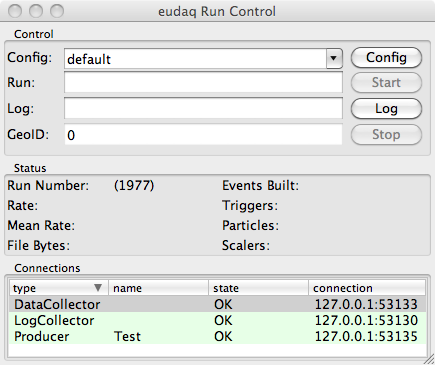
\includegraphics[width=0.6\textwidth]{RunControl}
    \caption{The Run Control graphical user interface.}
    \label{fig:RunControl}
  \end{center}
\end{figure}

Normally no command-line options should be needed, but it can be told to listen on a non-standard port,
(e.g. to run two copies on the same machine), with the \texttt{-a \param{port}} option:
\begin{listing}[mybash]
$[./euRun.app/Contents/MacOS/euRun]$ -a 3000
\end{listing}

This example is for Mac OS X, where the executable is inside an application bundle,
on other architectures it will be just \texttt{euRun.exe}.
Note also that it is not recommended to run two copies of the DAQ simultaneously,
since it becomes difficult to keep them completely separate as the Log and Data Collectors
must also be run on different ports.

\subsubsection{Log Collector}
Running the Log Collector is optional. If it is run, then all log messages generated by all other processes
in the DAQ will be collected in one central location.

\begin{figure}[htb]
  \begin{center}
    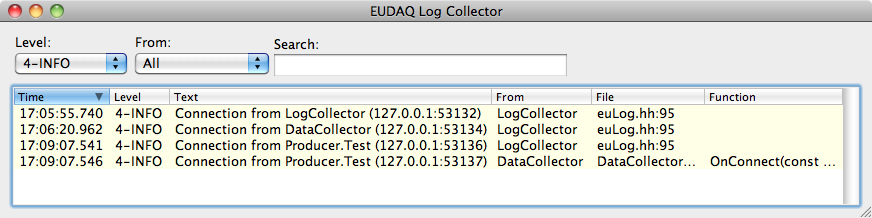
\includegraphics[width=\textwidth]{LogCollector}
    \caption{The Log Collector graphical user interface.}
    \label{fig:LogCollector}
  \end{center}
\end{figure}

Like the Run Control, there are also two versions of the Log Collector.
The graphical version is called \texttt{euLog.exe}, or \texttt{euLog.app} on Mac OS X,
and the text-based version is called \texttt{TestLogCollector.exe}.

If it is being run on the same machine as the Run Control, it should not need any command-line options.
However, if it is run on a different machine, it must be told on which machine the Run Control is running,
using the \texttt{-r \param{hostname}} option, e.g.:
\begin{listing}[mybash]
$[./euLog.exe]$ -r eudetmac001.cern.ch
\end{listing}

It may also be told to listen on a non-standard port, using the \texttt{-a \param{port}} option, similar to the Run Control.

\subsubsection{Data Collector}
The Data Collector is the process that collects all the raw data from the Producers,
merges all the incoming streams into a single data stream, and writes it to file.

Like the Log Collector, it should be told where to connect to the Run Control if it is not running on the same machine,
and it may also be told to listen on a non-standard port, with the \texttt{-r} and \texttt{-a} options respectively, for example:
\begin{listing}[mybash]
$[./TestDataCollector.exe]$ -r eudet
\end{listing}

\subsubsection{TestProducer}
For testing purposes, you may use the Test Producer.
This works similarly to a real producer, but does not talk to any real hardware,
instead providing a menu for the user to manually send events
(or see the ExampleProducer, below).

\subsubsection{ExampleProducer}
The ExampleProducer was written to illustrate the writing of a new Producer (see \autoref{sec:Producers}).
However, it will actually generate some example data, and so can also be used for testing purposes.
It works more like a real Producer than the TestProducer,
in that it does not require user intervention to generate each trigger,
and the data generated emulates a simple (but realistic) sensor,
and can be properly converted, and therefore displayed in the Monitor.

\subsubsection{TLUProducer}
If you do not have a \gls{TLU} in your setup, you may skip this part.
Otherwise you should run a TLUProducer, which will configure the \gls{TLU},
and read out the timestamps and send them to the Data Collector.

On the computer with the \gls{TLU} connected, start the \texttt{TLUProducer.exe} program.
If this is not the same machine as the Run Control,
use the \texttt{-r} option as for the Data and Log Collectors.
For example:
\begin{listing}[mybash]
$[./TLUProducer.exe]$ -r eudet.unige.ch:3000
\end{listing}

If the TLUProducer fails to start, make sure the permissions are set up correctly (see \autoref{sec:TLUperm}).

\subsubsection{EUDRBProducer}
The \gls{EUDRB} boards are used to read out the telescope sensors.
The \gls{EUDRB} Producer is designed to run on a Motorola MVME6100 single board computer,
using the Tundra TSI148 VME bridge for communication with the \glspl{EUDRB}.

If more than one EUDRBProducer is to be run, they must all have different names.
The name can be set with the \texttt{-n \param{name}} option.

As with the other processes, the address of the Run Control should be set with the \texttt{-r} option.
An example is shown below:
\begin{listing}[mybash]
$[./EUDRBProducer.exe]$ -n EUDRB2 -r 192.168.1.1
\end{listing}

\subsubsection{Other Producer(s)}
If you have a producer for your own hardware (see \autoref{sec:Producers}),
it should also have an option to set the address of the Run Control.

\subsubsection{RootMonitor}

\begin{figure}[htb]
  \begin{center}
    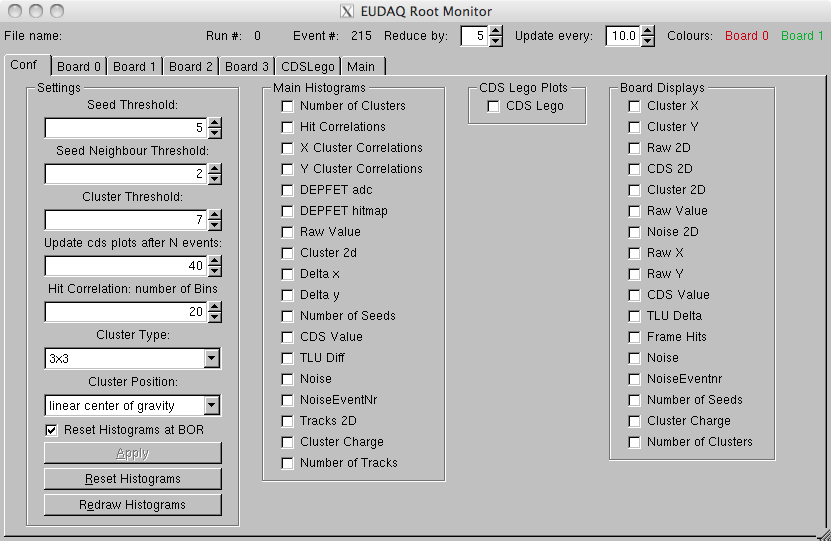
\includegraphics[width=0.9\textwidth]{RootMonitorConf}
    \caption{The Root Monitor configuration screen.}
    \label{fig:RootMonitorConf}
  \end{center}
\end{figure}

The RootMonitor reads the data file written by the Data Collector,
and generates several Root histograms that can be useful for online monitoring.
Since it reads the native data file directly, it must be run on the same machine as the Data Collector.

Although all plots are always generated internally by the Root Monitor,
you can configure which plots are displayed on screen.
The \texttt{Conf} tab (see \autoref{fig:RootMonitorConf}) contains four groups:
\texttt{Settings}, where various parameters of the plots may be configured,
\texttt{Main Histograms} for selecting which plots to show on the \texttt{Main} tab,
\texttt{CDS Lego Plots} to select whether to show Lego plots of the per-board CDS profiles,
and \texttt{Board Displays} to select which plots to display on the per-board tabs.
After making any changes the \texttt{Apply} button must be pressed for them to take effect.
\autoref{fig:RootMonitorPlots} shows an example of a per-board display with 2D, x and y cluster profiles,
cluster charge and number distributions, and a 2D \gls{CDS} profile.

\begin{figure}[htb]
  \begin{center}
    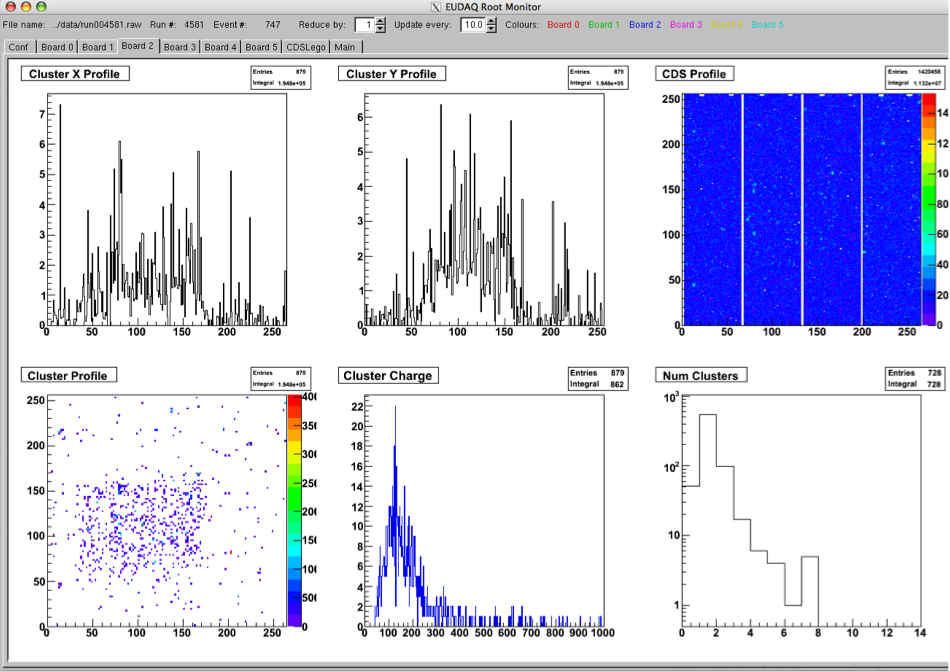
\includegraphics[width=0.8\textwidth]{RootMonitorPlots}
    \caption{The Root Monitor showing some online plots.}
    \label{fig:RootMonitorPlots}
  \end{center}
\end{figure}

Due to the way the Root Monitor is implemented,
it does not have access to the data file at the time the histograms are booked.
This is a problem, since depending on what is in the data file,
the number and parameters of the histograms may vary.
To work around this, a simple text configuration file is used to specify these parameters.
It is called \texttt{rootmonitor.conf},
and is located in the directory from which the RootMonitor is run (usually \texttt{bin}).
The file should contain one line per sensor in the data file,
and may also contain comments (lines starting with a \texttt{\#} character).
Each sensor line has a number of parameters, separated by commas,
and all apart from the first are optional.
These are: sensor type, width, height, pedestal file, seed threshold,
neighbour threshold, cluster threshold, cluster size.
Where width and height are in pixels, and the thresholds are in ADC units,
and are used for clustering.

The RootMonitor can be run in one of two modes: online or offline.
In online mode, it connects to the RunControl, so it will know when new runs are started,
and it will automatically open each new data file as it is created.
In offline mode, there is no Run Control,
and it only analyses the data file it is given on the command line. 
An example command line is:
\begin{listing}[mybash]
$[./RootMonitor.exe]$ -f 5432
\end{listing}

This will run it in offline mode, opening the file corresponding to run 5432
(alternatively, the full path to a file may be given).
To run it in online mode, simply omit the \texttt{-f} option,
then the \texttt{-r} option may be used if the Run Control
is running on a different computer or using a non-standard port.

\subsection{Running the DAQ}
To start the DAQ, all the necessary processes must be started in the correct order.
The first process must be the Run Control,
since all other processes will attempt to connect to it when they start up.
Then it is recommended to start the Log Collector,
since any log messages it receives may be useful
to help with debugging in case everything does not start as expected.
Next, the Data Collector should be started.
Finally all the Producers, and if needed, the RootMonitor.

\subsubsection{STARTRUN}\label{sec:STARTRUN}
The \texttt{STARTRUN} file, in the main \texttt{eudaq} directory
(as opposed to the \texttt{bin} subdirectory where the executables exist),
is a shell script that can be customized to load the appropriate processes for running the DAQ.
This allows you to start all the processes necessary with a single command.
If starting processes on other computers via SSH,
it is recommended to set up SSH keys so that the processes may be started without having to type a password.

In the future the \texttt{STARTRUN} script may be replaced with a more intelligent version
that uses a configuration file generated by the config script to decide what to load.

\subsubsection{Controlling the DAQ}
Once all the processes have been started, the DAQ can be configured, and runs may be started and stopped
using the Run Control (see \autoref{fig:RunControl}).

First the appropriate configuration should be selected from the drop-down list
(see \autoref{sec:ConfigFiles} for creating and editing configurations),
and the \texttt{GeoID} should be verified (see \autoref{sec:GeoID}), before continuing.

Then the \texttt{Config} button can be pressed,
which will send a configuration command
(with the contents of the selected configuration file) to all connected processes.
The full contents of the configuration file will also be stored
in the \gls{BORE} of the data file,
so that this information is always available along with the data.

Once all connected processes are fully configured, a run may be started, by pressing the \texttt{Start} button.
Whatever text is in the corresponding text box when the button is pressed
will be stored as a comment in the data file.
This can be used to help identify the different runs later.

Once a run is completed, it may be stopped by pressing the \texttt{Stop} button.
Runs will also stop and restart automatically when the data file reaches a threshold in size
(by default this is 1~GB).
This is because there is a file size limit of 2~GB for storage on the GRID,
and the processed files can grow bigger than the original native files.
The threshold size for restarting a run may be configured in the config file (see \autoref{sec:ConfigFiles}).

At any point a message may be sent to the log file by filling in the \texttt{Log} text box and pressing the corresponding button.
The text should appear in the LogCollector window, and will be stored in the log file for later access.

Once the run is stopped, the system may be reconfigured with a different configuration, or another run may be started.

\subsubsection{Config Files}\label{sec:ConfigFiles}
The \texttt{Config} drop-down in the Run Control is populated from the files in the \texttt{config} subdirectory.
These are just text files in a specific format, containing name-value pairs separated into different sections.
See \autoref{sec:ExampleConfig} for an example file.

Any text from a \texttt{\#} character until the end of the line is treated as a comment, and
ignored.  Each section in the config file is delimited by a name in square brackets
(e.g. \verb@[RunControl]@).  The name represents the type of process to which it applies; if there
are several such processes, then they can be differentiated by including the name after a period
(e.g. \verb@[Producer.Example]@).  Within each section, any number of parameters may be specified,
in the form \mbox{\texttt{Name = Value}}.  It is then up to the individual processes how these
parameters are interpreted.

The entire contents of the config file will be sent to all processes during the configuration, and
each process will have the appropriate section selected.  The file will also be attached to the
\gls{BORE}, so that it is available with the data later, even if the original config file is
modified or deleted.

\subsubsection{GeoID}\label{sec:GeoID}
The GeoID is a number representing the physical positioning of the telescope and DUT(s).
Each time a change is made to the telescope layout, this number should be incremented.
To change the number, double-click on it, and a window will appear with the new value.
By default it will increment the old value by one, so normally you should just click \texttt{OK},
but if necessary you may edit the value first.

The GeoID is inserted into the config file when it is sent, so it is also stored in the data file,
and will be used to select the correct GEAR file for alignment during the data analysis stage.

\subsection{Other Utilities}
There are a number of other utilities available that are not needed for running the DAQ,
but can be useful for other tasks such as debugging.
The executables are all located in the \texttt{bin} subdirectory.
They should all accept a help (\texttt{-h} or \texttt{--help}) option,
to print a summary of the available options.

\subsubsection{TLUControl}
The \texttt{TLUControl.exe} program is a standalone program for running the TLU without using the
full DAQ. The most commonly used parameters are shown below. For each option, the short (preceeded
by one dash) and the long (preceeded by two dashes) option names are shown (only one of the two
forms should be used for each option, but long and short options can be mixed together on the
command line), along with any parameters and their default value that will be used if the option is
not specified.

\begin{description}
\ttitem{-d --dutmask \param{mask = 0}}
The DUT mask; this defines which DUT connections are activated.  It is a bit-mask, so 1 means
connector 0, 2 means connector 1, etc..

\ttitem{-a --andmask \param{mask = 255}}
The AND mask; this defines which external trigger inputs are activated. It is a bit-mask, so 1
means channel 0, 2 means channel 1, etc.. The specified channels are ANDed together, and used to
generate a trigger signal.

\ttitem{-t --trigger \param{msecs = 0}}
Internal trigger period.  If non-zero, the \gls{TLU} will generate internal triggers with the
specified period in milliseconds. If set to zero, the internal trigger is off.

\ttitem{-i --dutinputs \param{values = ""}}
Input mode select. A sequence of comma-separated strings specifying which connectors to use for the
DUT inputs. Valid values are \texttt{RJ45}, \texttt{LEMO}, \texttt{HDMI}, and \texttt{NONE}.

\ttitem{-u --wait-for-user}
Pause the program after the \gls{TLU} is configured, before starting triggers. The default is to not
wait for the user.
\end{description}

Other parameters available are as follows:

\begin{description}
\ttitem{-o --ormask \param{mask = 0}}
The OR mask; this defines which external trigger inputs are activated. It is a bit-mask, so 1
means channel 0, 2 means channel 1, etc.. The specified channels are ORed together, and used to
generate a trigger signal.

\ttitem{-v --vetomask \param{mask = 0}}
The VETO mask; this defines which external trigger inputs are activated. It is a bit-mask, so 1
means channel 0, 2 means channel 1, etc.. The specified channels are used to veto the generation
of a trigger if they are active.

\ttitem{-w --wait \param{ms = 1000}}
Wait time. This is the time to wait between updates.

\ttitem{-n --notimestamp}
Indicates that the timestamp buffer should not be read out.

\ttitem{-q --quit}
Quit the program after configuring the TLU.

\ttitem{-s --save-file \param{filename = ""}}
     The filename to save trigger numbers and timestamps

\ttitem{-p --strobeperiod \param{cycles = 1000}}
Period for timing strobe (in \gls{TLU} clock cycles).

\ttitem{-l --strobelength \param{cycles = 100}}
Length of `on' time for timing strobe (in \gls{TLU} clock cycles).

\ttitem{-b --dutveto \param{mask = 0}}
Mask for enabling veto of triggers (`backpressure') by rasing DUT\_CLK.

\ttitem{-hm --handshakemode \param{nohandshake = 0}}
In this mode the TLU issues a fixed-length pulse on the trigger line (0 = no handshake).

\ttitem{-pw --powervctrl \param{mV = 800}}
[obsolete but provided for backward compatibility, please use \texttt{-pv}] Sets the Vcntl control
voltage to all PMTs. The range of values is between 0 and 1000 (or 0 and 2000 if the \gls{TLU} has
been modified by cutting \texttt{LC1} and jumpering \texttt{LO1} on the PMT Supply Daughterboard and
specifying the \texttt{-pm 1} option).

\ttitem{-pv --pmtvcntl \param{mV = 800}}
Sets the Vcntl control voltage to all PMTs (see option \texttt{-pw} for more details). Will override
the value of \texttt{-pw} if it is specified. If neither \texttt{-pw} or \texttt{-pv} is specified,
the default value will be used (and can be overridden on an individual PMT basis).

\ttitem{-p1 --pmtvcntl1 \param{mV}}
Sets the PMT Vcntl voltage for PMT1 (Chan 0) only. If not specified, the default or values specified
by \texttt{-pw} or \texttt{-pv} (which will override \texttt{-pw}) is used.

\ttitem{-p2 --pmtvcntl2 \param{mV}}
Sets the PMT Vcntl voltage for PMT2 (Chan 1) only. If not specified, the default or values specified
by \texttt{-pw} or \texttt{-pv} (which will override \texttt{-pw}) is used.

\ttitem{-p3 --pmtvcntl3 \param{mV}}
Sets the PMT Vcntl voltage for PMT3 (Chan 2) only. If not specified, the default or values specified
by \texttt{-pw} or \texttt{-pv} (which will override \texttt{-pw}) is used.

\ttitem{-p4 --pmtvcntl4 \param{mV}}
Sets the PMT Vcntl voltage for PMT4 (Chan 3) only. If not specified, the default or values specified
by \texttt{-pw} or \texttt{-pv} (which will override \texttt{-pw}) is used.

\ttitem{-pm --pmtvcntlmod \param{value = 0}}
Specifies whether the TLU PMT Supply Daughtercard is modified (\texttt{LC1} cut and \texttt{LO1}
jumpered) or not.  A \param{value} of 0 specifies that it is unmodified (and thus the Vcntl range is
from 0mV to 1000mV), and a \param{value} of 1 specifies that the \gls{TLU} is modified (and thus the
Vcntl range is from 0mV to 2000mV).  This feature is to accomodate newer Hamamatsu PMT models
(e.g. H10721) that require a control voltage range of, for instance, 500mV to 1100mV that are being
used in place of the older (discontinued, but what the \gls{TLU} was designed to accomodate and
control) models that required a control voltage of between 250mV and 900mV.

\ttitem{-f --bitfile \param{filename = ""}}
The bitfile containing the TLU firmware to be loaded.

\ttitem{-e --error-handler \param{value = 2}}
Error handler setting. Setting to 0 indicates the program should abort on an error. Setting it to a
value greater than 0 indicates the number of tries that should be attempted before generating an
exception.

\ttitem{-r --fwversion \param{value = 0}}
Specifies the firmware version to load (setting to 0 indicates the version should be chosen automatically).

\ttitem{-z --trace-file \param{filename = ""}}
The filename to save a trace of all USB accesses. Prepend a dash (`\texttt{-}') to output errors
only, or a plus (`\texttt{+}') for all data (including block transfers).
\end{description}

An example use of the command is shown below:

\begin{listing}[mybash]
$[./TLUControl.exe]$ -t 200 -d 3 -i LEMO,RJ45 -u
Using options:
TLU version = 0 (auto)
Bit file name = '' (auto)
Trigger interval = 200 ms (5 Hz)
DUT Mask  = 0x03 (3)
Veto Mask = 0x00 (0)
And Mask  = 0xff (255)
Or Mask   = 0x00 (0)
DUT inputs = LEMO,RJ45
Strobe period = 0x0003e8 (1000)
Strobe length = 0x000064 (100)
Enable DUT Veto = 0x00 (0)
Save file = '' (none)

TLU Version = v0.2c
TLU Serial number = 0x062b (1579)
Firmware file = TLU2_Toplevel.bit
Firmware version = 65
Library version = 65

Press enter to start triggers.

TLU Started!

Status:    20,00,--,--,--,-- (0,0)
Scalers:   0, 0, 0, 0
Particles: 2
Triggers:  0
Entries:   0
TS errors: 0, 0 (redundancy, re-read)
Timestamp: 0x8d768 (579432) = 0.00150891
Time: 0.009 s, Freq: 0 Hz, Average: 0 Hz

        0, 0x27fb479 (41923705) = 0.109174, diff=41923705
        1, 0x7139ab9 (118725305) = 0.309174, diff=76801600
        2, 0xba780f9 (195526905) = 0.509174, diff=76801600
        3, 0x103b6739 (272328505) = 0.709174, diff=76801600
        4, 0x14cf4d79 (349130105) = 0.909174, diff=76801600
Status:    20,00,--,--,--,-- (0,1)
Scalers:   0, 0, 0, 0
Particles: 7
Triggers:  5
Entries:   5
TS errors: 0, 0 (redundancy, re-read)
Timestamp: 0x1726fa48 (388430408) = 1.01152
Time: 1.023 s, Freq: 4.92913 Hz, Average: 4.88442 Hz

        5, 0x196333b9 (425931705) = 1.10917, diff=76801600
        6, 0x1df719f9 (502733305) = 1.30917, diff=76801600
        7, 0x228b0039 (579534905) = 1.50917, diff=76801600
        8, 0x271ee679 (656336505) = 1.70917, diff=76801600
        9, 0x2bb2ccb9 (733138105) = 1.90917, diff=76801600
Status:    20,00,--,--,--,-- (0,1)
Scalers:   0, 0, 0, 0
Particles: 12
Triggers:  10
Entries:   5
TS errors: 0, 0 (redundancy, re-read)
Timestamp: 0x2e5bb708 (777762568) = 2.02538
Time: 2.037 s, Freq: 4.93259 Hz, Average: 4.90838 Hz
^CQuitting...
\end{listing}

This sets up internal triggers at 5~Hz (200~ms period), and activates DUT inputs 0 and 1.
Input 0 is configured to use the LEMO connector, and input 1 to use the RJ45 connector.
The first part of the output just summarizes the input parameters.
The next part shows information about the version numbers of the TLU and the firmware.

It will then configure the \gls{TLU}, and if the \texttt{-u} option is used,
it will wait for the user to press enter before continuing.
The triggers are then enabled, and a summary of the status is printed out periodically
(by default every 1~second).
The program can be stopped cleanly by pressing \texttt{Ctrl-C}.

Each block of status output consists of:
\begin{myitemize}
\item a list of triggers, if there were any since the last update (the first time there are none),
each showing:
  \begin{myitemize}
  \item the trigger number,
  \item the timestamp of the trigger, in hex, decimal and converted to seconds,
  \item the difference since the last trigger.
  \end{myitemize}
\item the status of the \gls{DUT} connections (see below),
\item the values of the scalers on the external trigger inputs,
\item the number of ``particles'', which means all the potential triggers (including those that were vetoed),
\item the number of triggers that actually got sent to the \glspl{DUT},
\item the number of entries in the trigger buffer,
this should be equal to the number of triggers printed out at the top of the status block,
\item the number of timestamp errors detected by redundancy, and by re-reading,
\item the current timestamp value,
\item the time since the run started, the current trigger frequency, and the average frequency over the whole run.
\end{myitemize}

In the example output this block is repeated three times, before \texttt{Ctrl-C} is pressed to stop it.
The status is of the \gls{DUT} connections formatted as:
\begin{myitemize}
\item two digits for each \gls{DUT} connection consisting of:
  \begin{myitemize}
  \item two hyphens (\texttt{--}) if the connection is inactive, else
  \item the first digit represents the inputs from the \gls{DUT}; with the busy line in bit 0 and the clock line in bit 1
  (note the clock input can float low or high if a LEMO input is selected, as it is not connected),
  \item the second digit represents the state of the FSM, as defined in the \gls{TLU} manual\cite{Cussans2009}
  (0 is ready, 1 is waiting for busy high, 4 is waiting for busy low, 5 is \gls{DUT}-initiated veto, and F is an error condition).
  \end{myitemize}
\item then in parentheses:
  \begin{myitemize}
  \item the veto state (software veto in bit 0, overall veto in bit 1),
  \item the DMA state (1 when a DMA transfer is taking place).
  \end{myitemize}
\end{myitemize}

\subsubsection{VMETest}
The VMETest.exe program uses the EUDAQ VME library to perform VME accesses.
It can be useful for determining whether a VME card is responding at a particular address.
The available options are:
\begin{description}
\ttitem{-b \param{address}}
The base address for the VME accesses.
This value will be added to the offsets specified in the commands to give the actual address used.

\ttitem{-s \param{bytes}}
Sets the window size in bytes.
This is the amount of memory that is mapped into the VME address space.
Any accesses outside this range will result in an access violation.

\ttitem{-a \param{bits}}
The address bus width in bits.
Valid values are 16, 24, 32 or 64.

\ttitem{-d \param{bits}}
The data bus width in bits.
Valid values are 8, 16, 32 or 64.

\ttitem{-m \param{mode}}
The VME access mode.
Valid values are S (single accesses), B (BLT), M (MBLT), 2 (2eVME), E (2eSST) and T (2eSSTB).

\end{description}

The options set up the mode for the VME accesses.
Following the options, a number of commands can be specified to perform actual reads or writes.
The commands can be any of the following:
\begin{description}
\ttitem{r\param{offset}}
Reads a value from the specified offset, and displays the value read.

\ttitem{R\param{offset},\param{words}}
Performs a block read of the specified number of words, starting from the specified offset.

\ttitem{w\param{offset},\param{value}}
Writes the specified value to the specified offset.

\ttitem{W\param{offset},\param{value1}{[},\param{value2}\ldots{]}}
Performs a block write of the specified values, starting at the specified offset.

\end{description}

Numerical arguments to either the options or the commands can be given either in decimal,
or in hexadecimal by prefixing them with \texttt{0x}, as in C or C++.
Note that the options require a space between the option character and its argument,
but the commands must not have a space.
For example:

\begin{listing}[mybash]
$[./VMETest.exe]$ -b 0x180000 -a 24 -d 16 w0x20,123 r0x10
\end{listing}

This sets up a window starting at 180000 hex, in A24 address space with D16.
It then writes the value 123 to offset 32 (20 hex), and then reads the value at offset 16 (10 hex).

\subsubsection{TestReader}\label{sec:TestReader}
The \texttt{TestReader.exe} program will read a native data file,
and can display various pieces of information from the file.
Commonly used options are:
\begin{description}
\ttitem{-b}
Display the \gls{BORE}.

\ttitem{-e}
Display the \gls{EORE}.

\ttitem{-d \param{range}}
Display the specified range of event numbers.

\ttitem{-p}
Process the displayed events and display the corresponding StandardEvents.

\ttitem{-u}
Dump the raw data for the displayed events.

\ttitem{-s}
Try to resynchronize events based on the \gls{TLU} event number.
A full description of this option is outside the scope of this manual
(but if you don't know what it is, you probably don't need it).

\end{description}

After the options a list of one or more filenames can be given.
Any filenames that consist only of numerical digits
will be interpreted according to the input pattern
(by default this is ``\texttt{../data/run\$6R.raw}'',
where \texttt{\$6R} will be replaced with the run number padded to 6 digits).
For example:
\begin{listing}[mybash]
$[./TestReader.exe]$ -b -e -p -d 1-10,100,1000 example.raw 5432
\end{listing}

This will display the \gls{BORE} and \gls{EORE}, and the events 1 to 10, 100 and 1000,
processing them to also display the StandardEvents,
from the files \texttt{example.raw} and \texttt{../data/run005432.raw}.

\subsubsection{Converter}\label{sec:Converter}
The \texttt{Converter.exe} program will read a native data file,
optionally select just a subset of events from the file,
and can then write it out to another file in either the same native format, or a different format.
The most commonly used options are:
\begin{description}
\ttitem{-t \param{type}}
The file type to write out.
The available types are listed below.

\ttitem{-e \param{range}}
Select the specified range of event numbers.

\ttitem{-s}
Try to resynchronize events based on the TLU event number
(see TestReader in \autoref{sec:TestReader}).

\end{description}

The available output file types are as follows:

\begin{description}\phantomsection\label{lst:FileTypes}

\ttitem{native}
The native EUDAQ binary file format, consisting of a serialised stream of
\texttt{DetectorEvent}s, containing the raw data read out from the hardware.

\ttitem{standard}
Like the \texttt{native} format, this is also a serialised stream,
but in this case it contains \texttt{StandardEvent}s,
in which the raw data has been converted into a standard format.

\ttitem{lcio}
The standard \gls{LCIO} file format used by the analysis software.
This type is only available if EUDAQ was compiled with \gls{LCIO} support.

\ttitem{root}
A Root file containing a TTree with the hit pixel information.

\ttitem{text}
A simple text based format (not yet implemented).

\ttitem{mimoloop}
A text based format mimicking the output of the mimoloop program
(from Angelo Cotta Ramusino and Lorenzo Chiarelli at INFN Ferrara).

\end{description}

Although this program can be used to convert a native data file into \gls{LCIO} format,
the more usual (and therefore better tested) way is to use the EUTelescope converter.

\subsubsection{ClusterExtractor}
This program can be used to quickly extract some clusters from raw data.
It is not as sophisticated as the EUTelescope package, which should be preferred for real analysis,
but it can be useful for doing quick checks, possibly with the \texttt{Correlator} (see below).
It will read a native data file, perform a basic clustering,
and then write these clusters to one text file per sensor plane.
The most commonly used options are:
\begin{description}
\ttitem{-p \param{pixels}}
The cluster size in pixels.
It should be an odd number, with 1 meaning no clustering (just pixels over threshold),
3 meaning 3\x{}3 pixel clusters, etc.

\ttitem{-n \param{adcs}}
The noise level (sigma) in ADC units.
This is used to scale the thresholds in terms of the noise.

\ttitem{-s \param{thresh}}
The threshold for seed pixels, in terms of the noise.

\ttitem{-c \param{thresh}}
The threshold for the total charge of a cluster,
in terms of the cumulative noise of all the pixels in the cluster.

\ttitem{-w}
Reports the cluster centre as the weighted average of the pixels,
instead of the position of the seed pixel.

\end{description}

An example use is:
\begin{listing}[mybash]
$[./ClusterExtractor.exe]$ -p 3 -n 3.5 -s 6 -c 10 -w 5432
\end{listing}

This will generate a number of text files named \texttt{runNNN\_eutel\_M.txt},
where \texttt{NNN} is the run number, and \texttt{M} is the sensor plane number.
The format of the output text files is as follows:
\begin{listing}[]
2       2       51487659237
 182    153     126
 241    120     125
3       1       51489095892
 111    67      346
5       1       51491334074
 113    141     171
7       2       51495330212
 252    240     305
 95     170     189
\end{listing}

The first line contains the event number,
the number of clusters, and the TLU timestamp.
Then for each cluster there is one line,
containing the \texttt{x} and \texttt{y} coordinates of the cluster centre,
and the total charge in ADC units.
The cluster lines are prepended with a space to make it easier to scan the file by eye.

\subsubsection{Correlator}
The \texttt{Corellator.exe} program is used to look for correlation between different sensor planes.
This can be a useful check that everything is properly aligned and synchronised.
It uses as input the text files generated by the \texttt{ClusterExtractor} program.
It can generate a number of plots that are saved to a Root file, and optionally displayed on screen.

\begin{figure}[htb]
  \begin{center}
    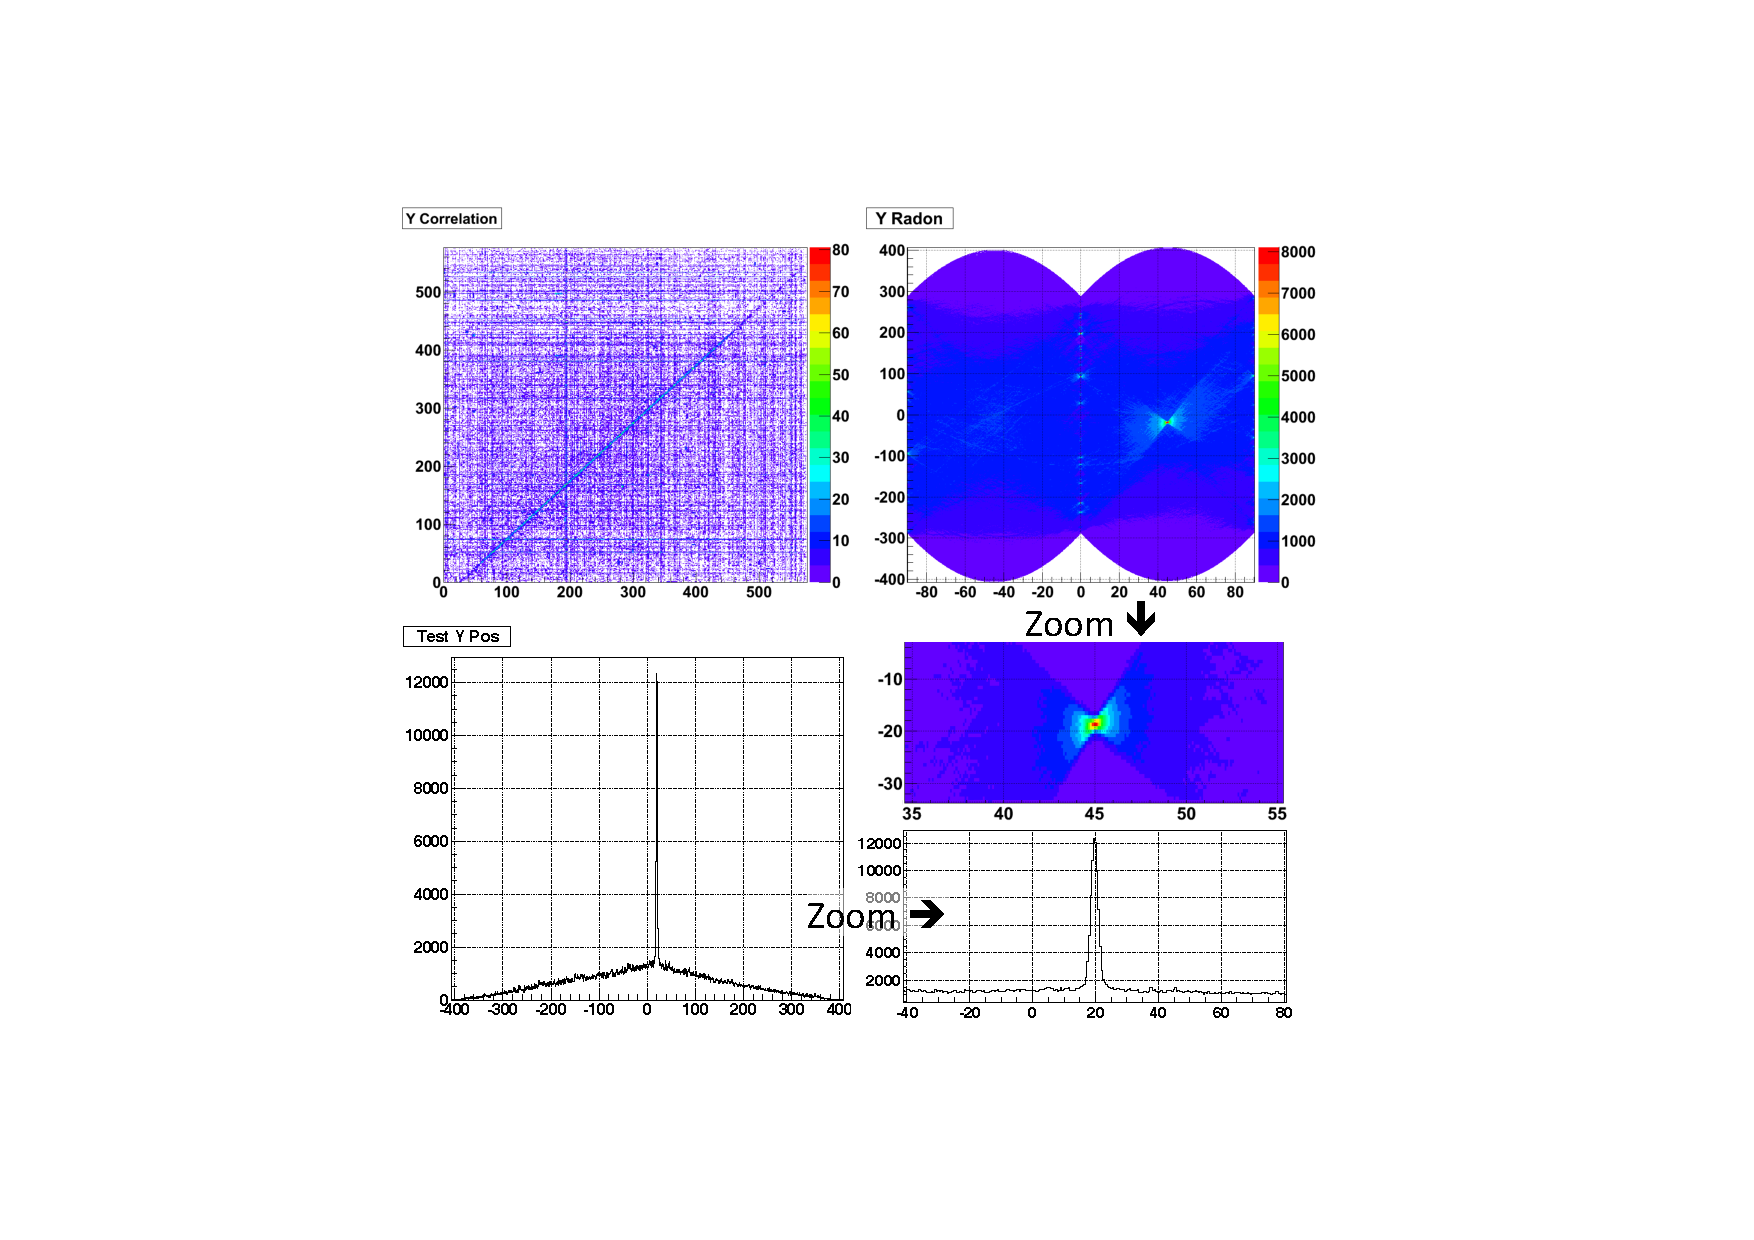
\includegraphics[width=0.7\textwidth]{correl}
    \caption{Correlation plots.}
    \label{fig:Correlation}
  \end{center}
\end{figure}

The basic correlation plot (\autoref{fig:Correlation}, top left) consists of looping over every pair of clusters for each given event,
and plotting the \texttt{x} (or \texttt{y}) coordinate of the first cluster against that of the second.
For clusters that come from the same track, these coordinates should be correlated,
giving a straight line on the 2D plot, while other pairs should be uncorrelated,
giving a more or less flat background.
The amount of background depends on the multiplicity of clusters;
with only one cluster per event there is only one possible pair, and no background.
As the multiplicity increases, so will the background.

The Radon plot (\autoref{fig:Correlation}, top right) is a transformation of the basic plot,
into a space where each point represents a straight line in the original plot,
with the x-axis representing the angle, and the y-axis the offset from the centre.
There should be a peak at the point representing the correlation line of the first plot
(see zoomed area).

Given the relative pitch of both sensors, the angle of the correlation line is known
(e.g. it will have a gradient of 1, or angle of 45\degree, if both sensors have the same pitch).
Therefore there is no need to calculate the full Radon transform,
but just a slice at the correct angle,
which is what is done in the third plot.
We can see it gives a relatively flat background level,
with a very sharp peak at a particular offset
that depends on the relative alignment of the two sensors.

The most used parameters for running the program are:
\begin{description}
\ttitem{-x\textit{N} / -y\textit{N} \param{pixels}}
Sets the width (x) or height(y) of the sensors, where \texttt{N}
is 1 for the first and 2 for the second sensor.
The second sensor only needs to be specified if it differs in dimension from the first.
The sizes are needed since the text files do not contain the sensor dimensions,
and the dimensions are needed when booking the histograms.

\ttitem{-p\textit{N} \param{size}}
Sets the pitch of the two sensors.
This is only needed for the 1D slice of the Radon plot (\texttt{-t} option).

\ttitem{-l \param{clusters}}
Limit to events with fewer than a certain number of clusters,
in order to reduce the background.

\ttitem{-r}
Generate a Radon transform of the correlation plot.

\ttitem{-t}
Generate a 1D slice of the radon transform at the angle corresponding
to the ratio of the pitches of the two sensors.

\ttitem{-d}
Display the generated plots on screen, as well as saving them to file.

\end{description}

An example usage is:
\begin{listing}[mybash]
$[./Correlator.exe]$ -x1 1152 -y1 576 -t -d run5432_eutel_1.txt run5432_eutel_2.txt
\end{listing}

This sets the sensor dimensions to 1152\x576 pixels,
generates the 1D Radon slice (but not the full Radon plot),
using two text files generated by the \texttt{ClusterExtractor} as input,
and displays the generated plots on screen.

\subsubsection{MagicLogBook}
This program is designed to extract as much information as possible from data files and log files,
in order to reconstruct a log book.
Despite its name, it is in fact not magical,
so it is preferable to keep a good log book during running,
rather than relying on this program to generate it later.

The available options are listed below:
\begin{description}
\ttitem{-f \param{fields}}
A list of fields to include in the output, in the form \texttt{name=value},
with multiple fields separated by commas.
If a predefined list is also specified these will be appended to the list.

\ttitem{-s \param{separator}}
The separator to use between fields in the output. The default is a tab character.

\ttitem{-h \param{string}}
A string that appears at the beginning of the header line (with the list of field names),
that can be used to differentiate it from the other lines. The default is an empty string.

\ttitem{-p {name}}
Use a predefined list of fields.
Currently available values are \texttt{normal} and \texttt{full}.

\ttitem{-o \param{file}}
The output filename. By default the standard output is used.

\end{description}

The easiest method of running is to use a predefined list of fields.
There are currently two predefined lists available: \texttt{normal} and \texttt{full}.
If neither of these are suitable, contact the EUDAQ maintainer,
as it may be possible to add more options.

The \texttt{normal} list includes:
\begin{myitemize}
  \item the run number,
  \item the config file name,
  \item the run start time,
  \item for the \glspl{EUDRB}:
  \begin{myitemize}
    \item the mode,
    \item the sensor type,
    \item whether they are running unsynchronized,
    \item the number of boards,
    \item and the firmware version.
  \end{myitemize}
  \item and for the \gls{TLU}:
    \begin{myitemize}
    \item the internal trigger interval,
    \item the AND mask,
    \item the DUT mask,
    \item and the firmware version.
  \end{myitemize}
\end{myitemize}

The \texttt{full} list includes all the values from the \texttt{normal} list,
plus the number of events in the run and the end of run time.
This is because these values can only be known by reading
the whole data file to the end, which is slow, especially for large data files.

If necessary, other information is available using custom fields,
although the syntax for these is a bit complicated,
since it is designed to be as flexible as possible at specifying any information in the data file.
In the future it may be redefined in order to simplify it if possible.
Therefore it is recommended to use a predefined list of fields where possible.
Custom fields are specified as a comma separated list of items in the form \texttt{name=value},
with the name being what will appear on the header line of the output,
and the value specifying what exactly to extract from the file.
The possible values are illustrated below, although not exhaustively:

\begin{mydescription}
  \ttitem{events$^\ast$} The number of events in the run.
  \ttitem{config} The configuration name, or:
  \begin{mydescription}
    \ttitem{config:section:key} The value of the \texttt{key} from the corresponding \texttt{section} in the config
    (e.g. \texttt{config:Producer.EUDRB:NumBoards}).
  \end{mydescription}
  \item{\texttt{bore}, \texttt{tlu}, \texttt{eudrb}, \texttt{eore}$^\ast$:} Something from the \gls{BORE},
  the \texttt{TLUEvent} or \texttt{EUDRBEvent} subevents of the \gls{BORE}, or the \gls{EORE}, respectively:
  \begin{mydescription}
    \ttitem{bore:.Run} The run number
    \ttitem{bore:\param{name}} Otherwise, if the second part does not start with a period, the value of the tag \param{name} is used
    (e.g. \texttt{tlu:DutMask} or \texttt{eudrb:MODE}).
  \end{mydescription}
  \ttitem{log} Something from the log file (not implemented yet).
\end{mydescription}

$^\ast$ items marked with an asterisk require reading the whole data file, and are therefore slow,
especially when large data files are involved.

Note that the \texttt{EUDRBEvent} is now deprecated, having been replaced by the \texttt{RawDataEvent},
but there is currently no way to specify this.

The \texttt{MagicLogBook} command is used as follows:

\begin{listing}[mybash]
$[./MagicLogBook.exe]$ -p normal ../data/*.raw
\end{listing}

This will produce an output similar to the following:
\begin{listing}[]
Run  Config     Mode Det Start                   U P Trg AND  DUT  Tfw Efw
6371 eudet-beam          2009-07-29 07:44:39.535 1 6   0 0xf  0x10 241
6372 eudet-beam          2009-07-29 08:03:05.079 1 6   0 0xf  0x10 241
6373 eudet-m26test       2009-07-30 09:57:45.157 1 6 255 0xff 0x12 241
6374 eudet-m26test       2009-07-30 10:00:45.205 1 6 255 0xff 0x12 241
6375 eudet-m26test       2009-07-30 10:05:38.625 1 6   1 0xff 0x12 241
6376 eudet-m26test       2009-07-30 10:10:00.107 1 6   1 0xff 0x12 241
6379 eudet-m26test       2009-07-30 10:13:05.322 1 6   1 0xff 0x12 241
\end{listing}

Note that the header row has been modified slightly to fit into the page width:
the \texttt{U} should be \texttt{UnSync}, \texttt{P} should be \texttt{Planes},
\texttt{Trg} should be \texttt{TriggerInterval}, \texttt{Tfw} should be \texttt{TLUfw},
and \texttt{Efw} should be \texttt{EUDRBfw}.
The columns \texttt{Mode}, \texttt{Det} and \texttt{EUDRBfw} are missing from the output
due to the fact that this information is now stored in a \texttt{RawDataEvent},
which is not currently accessible with this version of the program.

\subsubsection{Others}
Some programs that are less used (or recently added)
may not be described here.
If they look interesting, you can find out more about them
by running them with the help (\texttt{-h} or \texttt{--help}) option,
or by examining the source code.

% !TEX root = EUDAQUserManual.tex
\section{Writing a Producer}\label{sec:Producers}
In order to integrate a \gls{DUT} fully into the DAQ, it needs its own Producer.
A Producer is both a CommandReceiver and a DataSender,
meaning it receives commands from Run Control,
and it also sends events to the Data Collector.
A base class is provided that users may inherit from, to make this as easy as possible.
For example code, see \autoref{sec:ExampleProducer}.

\subsection{Configuration}
The \texttt{Configuration} class is a way of storing configuration information
in a way that is easily accessible, and can be saved to or loaded from a human-readable file
(see \autoref{sec:ConfigFiles}), and can be sent over the network.
It is defined in the following header:

\begin{listing}
#include "eudaq/Configuration.hh"
\end{listing}

The configuration consists of a number of sections,
each of which contains a list of name-value pairs.
The values are stored as strings, but they can be converted to/from arbitrary types.
Methods are provided to load from or save to file, to set the current section,
and to set or get configuration values.
An example use is shown below:

\begin{listing}
std::ifstream infile("../conf/ExampleConfig.conf");
eudaq::Configuration config(infile, "Producer.Example");
int param = config.Get("Parameter", 0);
std::cout << "Loaded config, param = " << param << std::endl;
config.Set("Parameter", param+1);
config.Set("OtherParam", "something");
std::ofstream outfile("Test.conf");
config.Save(outfile);
\end{listing}

This creates a configuration loaded from the file \texttt{../conf/ExampleConfig.conf},
selecting the \texttt{Producer.Example} section.
It then gets an integer parameter from the configuration and displays it.
Then it modifies the value of the parameter and sets another parameter,
before writing the configuration to the file \texttt{Test.conf}.

A configuration object will be received by the Producer during the configuration,
as described in \autoref{sec:OnConfigure}.

\subsection{Receiving Commands}
Whenever a command is received from the Run Control,
a corresponding member function of the Producer will be called by the code in the base classes.
In order to react to a command, the necessary code is simply put inside the corresponding method.
The \texttt{Producer} base class is declared by including the following header file:
\begin{listing}
#include "eudaq/Producer.hh"
\end{listing}

\subsubsection{OnConfigure}\label{sec:OnConfigure}
This method is called whenever a configure command is received from the Run Control.
The method signature is:
\begin{listing}
virtual void OnConfigure(const eudaq::Configuration & config);
\end{listing}

As a parameter, it receives the configuration chosen in the Run Control.
Information may be extracted from the configuration in order to set up the hardware.

\subsubsection{OnStartRun}
This is called on the start of each run.
The method signature is:
\begin{listing}
virtual void OnStartRun(unsigned param);
\end{listing}

As a parameter, it receives the run number of the started run.
The Producer must send a \gls{BORE},
and then prepare for reading out events from the hardware.

\subsubsection{OnStopRun}
This is called at the end of the run.
The method signature is simply:
\begin{listing}
virtual void OnStopRun();
\end{listing}

Care should be taken that there are no more events pending to be read out.
Once all data events have been sent, an \gls{EORE} should also be sent,
to signal to the DAQ that the Producer has ended the run successfully.

\subsection{Sending Data and the RawDataEvent class}
Events may be sent to the DAQ using the \texttt{Producer}'s \texttt{SendEvent()} method
that has the following signature:
\begin{listing}
void SendEvent(const Event &);
\end{listing}

It takes as a parameter an object derived from the \texttt{eudaq::Event} base class
that will be serialised and sent to the Data Collector.
In practice it will usually be of concrete type \texttt{RawDataEvent}.

The \texttt{RawDataEvent} is a generic container for blocks of raw bytes,
used to encapsulate the data read out from the sensor electronics
and send it to the DAQ.
Each \texttt{RawDataEvent} may contain any number of raw data blocks.
By convention each block usually corresponds to one sensor,
but this is not required;
it is up to each Producer how the raw data are encoded,
since it is up to the corresponding DataConverterPlugin how they are decoded.
The RawDataEvent class is defined in the following header file:
\begin{listing}
#include "eudaq/RawDataEvent.hh"
\end{listing}

The class is described in more detail below.

\subsubsection{Constructing}
A \texttt{RawDataEvent} is constructed as follows:
\begin{listing}
RawDataEvent event("EXAMPLE", run, event);
\end{listing}

Where \texttt{"EXAMPLE"} is a string unique to the particular producer
that will be used to select the correct converter during decoding.
The \texttt{run} and \texttt{event} parameters are the run number
and event number respectively.

As well as normal data events, the producer must also send a \gls{BORE}
and \gls{EORE} at the beginning and end of a run respectively.
These are just normal \texttt{RawDataEvent} objects, but with a particular flag set.
The \texttt{RawDataEvent} has factory methods to simplify these cases:
\begin{listing}
RawDataEvent::BORE("EXAMPLE", run);
RawDataEvent::EORE("EXAMPLE", run, event);
\end{listing}

These methods return a \texttt{RawDataEvent} that may be either be sent directly to the DAQ,
or be modified first, e.g. by setting tags as described below in \autoref{sec:Tags}.

\subsubsection{Adding Data}
Once a RawDataEvent has been constructed,
data blocks may be added either using a vector:
\begin{listing}
std::vector<unsigned char> buffer = ...;
event.AddBlock(id, buffer);
\end{listing}

or using a pointer to a block of memory, and a length in bytes:
\begin{listing}
unsigned char * buffer = ...;
event.AddBlock(id, buffer, len);
\end{listing}

Where \texttt{id} is an integer used to differentiate the different blocks.
Usually it can just be 0 for the first block and increment by 1 for the following blocks.
And \texttt{buffer} contains the actual data for the block.
If the buffer is a \texttt{vector}, the whole length is used,
if it is a pointer, then the length must be specified.

The type of the vector or pointer need not be \texttt{unsigned char},
since these methods are in fact template methods that can take a vector of any basic type,
but if larger types are used, care must be taken about endianness,
since the buffer will be converted to \texttt{unsigned char}
according to the endianness of the machine it is running on.
Therefore if the producer may run on different architectures steps should be taken
to ensure that any endianness issues are handled correctly.

\subsubsection{Tags}\label{sec:Tags}
The \texttt{RawDataEvent} (in fact any type that descends from the \texttt{Event} base class)
may also have tags set.
These are name-value pairs containing extra information that does not easily fit
in the usual raw data.
This is used particularly in the \gls{BORE} to include information about the particular run
that may be useful for the decoding later.
A tag may be set as follows:
\begin{listing}
event.SetTag("Temperature", 42);
\end{listing}

The value corresponding to the tag can be set as an arbitrary type (in this case an integer),
it will be converted to a string internally.

\subsection{Log Messages}
A method is provided for sending log messages to the central Log Collector.
To use it the follwing header should be included:
\begin{listing}
#include "eudaq/Logger.hh"
\end{listing}

This defines the following macros for sending log messages,
listed in decreasing order of severity:
\begin{description}

\ttitem{EUDAQ\_USER}
A user-generated message (e.g. from the RunControl Log button).

\ttitem{EUDAQ\_ERROR}
Something that has gone wrong and should probably be looked into.

\ttitem{EUDAQ\_WARN}
A warning that something may not be quite right.

\ttitem{EUDAQ\_INFO}
An message generated during normal running containing information that may be useful to the user.

\ttitem{EUDAQ\_EXTRA}
Some extra information that may be less useful in normal running.

\ttitem{EUDAQ\_DEBUG}
Information for debugging purposes that will normally be hidden.

\end{description}

They are used as follows:
\begin{listing}
EUDAQ_ERROR("No keyboard detected: press F1 to continue.");
\end{listing}

The messages will be sent to the central Log Collector if it is connected,
otherwise they will be displayed on the local terminal.
The log level can be changed in the following way:
\begin{listing}
EUDAQ_LOG_LEVEL("WARN");
\end{listing}

Any messages lower than the specified level will just be ignored.
This can be useful to filter out unimportant messages and, for example, just display error messages.

% !TEX root = EUDAQUserManual.tex
\section{Data Conversion}
Data are stored on disk, by default, in a native binary format, containing the raw data as read out by the various Producers.
It is basically the same format used for serialising the data over the socket connection to the Data Collector.
To be useful, this data must be converted into a standardised format so that the monitoring and analysis software
does not depend on particularities of the individual sensors, but can be applied generically to any sensor.
Two different formats are used for this. The first is the \texttt{StandardEvent} type,
an internal class that does not depend on any external libraries,
and is used by the online monitoring, and many of the utility programs of the framework.
The second type is the \gls{LCIO} standard format from the linear collider community,
used by the full analysis software.

\subsection{StandardEvent and StandardPlane}
The \texttt{StandardEvent} is a class designed to represent pixel sensor data in a reasonably easy to use way,
but still be flexible enough to store the data from a wide range of different sensors as completely as possible.
Each \texttt{StandardEvent} represents one event of data from the whole telescope and any \glspl{DUT},
so a run will consist of a sequence of \texttt{StandardEvent}s.
It inherits from the \texttt{Event} base class, meaning that it has a run number, an event number, an optional timestamp,
and may also contain tags (see \autoref{sec:Tags}).
It also has an array of \texttt{StandardPlane}s, each representing one sensor plane of the telescope or \gls{DUT}.

Each \texttt{StandardPlane} contains the charge values from the pixels of one sensor,
and may contain several frames in cases where the sensor is read out multiple times per event.
It also has the concept of a ``result'' frame, which is calculated from the one or more of the source frames
according to different rules that may be specified with flags.
The result frame contains only one charge value per pixel, with a positive signal,
and is what will be used for the analysis.
It may consist of either differences between the original frames (e.g. in the case of \gls{CDS}),
a sum of all original frames, or specific parts of the different frames selected according to the pivot information.
Flags may be set to select which of the different methods is used.
It may also contain a submatrix number per pixel, which can be used to differentiate different parts of the sensor,
so that they may be analyzed separately later, and a pivot boolean (true or false) per pixel,
which can be used to indicate whether the pixel was sampled before or after the trigger,
and is used to determine which parts of the sensor to combine when the \texttt{FLAG\_NEEDCDS} flag is set.

Both the \texttt{StandardEvent} and the \texttt{StandardPlane} classes are defined in the following header file:
\begin{listing}
#include "eudaq/StandardEvent.hh"
\end{listing}

In general, a user should not need to construct a \texttt{StandardEvent} object,
but should create one or more \texttt{StandardPlane}s, that will be added to a given \texttt{StandardEvent}.

\subsubsection{Constructor}
The \texttt{StandardPlane} constructor has the following signature:
\begin{listing}
StandardPlane(unsigned id, const std::string & type,
              const std::string & sensor = "");
\end{listing}

Where \texttt{id} is an arbitrary numerical identifier for the plane
that can be used to differentiate between different planes of the same type,
\texttt{type} is the type of the Producer that generated the frame
(should be the same as that in the \texttt{Producer} and the \texttt{DataConverterPlugin}),
and \texttt{sensor} is the name of the sensor,
in the case that the Producer can read out more than one type of sensor.

\subsubsection{SetSizeRaw and SetSizeZS}
Once a \texttt{StandardPlane} has been constructed, the size should be set.
There are two methods for doing this,
depending on whether the data are stored in raw or zero-suppressed mode.
In raw mode all pixels are stored, whether they have a signal or not.
In zero-suppressed mode, only those with a signal above a certain threshold are stored,
along with their coordinates, and any below the threshold are suppressed.

The signature of the \texttt{SetSizeRaw} method is:
\begin{listing}
void SetSizeRaw(unsigned w, unsigned h, unsigned frames = 1, int flags = 0);
\end{listing}

Where \texttt{w} is the full width of the sensor (in the x-direction, usually columns) in pixels,
h is the full height of the sensor (in the y-direction, usually rows) in pixels, \texttt{frames} is the number of frames,
and \texttt{flags} may be a combination of the following values, separated by a bitwise OR (i.e. \texttt{|}):

\begin{description}
\ttitem{FLAG\_NEEDCDS} Indicates that the data are in 2 or 3 frames
and that neighbouring frames should be subtracted to produce the result.

\ttitem{FLAG\_NEGATIVE} Indicates that the charge values are negative,
so should be negated to produce the result.

\ttitem{FLAG\_ACCUMULATE} Indicates that all frames should be summed to produce the result.

\ttitem{FLAG\_WITHPIVOT} Indicates that pivot information is stored per pixel,
and should be used for constructing the result.

\ttitem{FLAG\_WITHSUBMAT} Indicates that submatrix information is stored per pixel.

\ttitem{FLAG\_DIFFCOORDS} Indicates that each frame can have different coordinates,
in the case of zero-suppressed data, otherwise all frames will share the same coordinates.

\end{description}

The signature of the \texttt{SetSizeZS} method is a follows:
\begin{listing}
void SetSizeZS(unsigned w, unsigned h, unsigned npix,
               unsigned frames = 1, int flags = 0);
\end{listing}

Where all parameters are the same as in \texttt{SetSizeRaw}, but there is an extra parameter (\texttt{npix})
that specifies how many pixels to preallocate.
If the number of pixels above threshold is known, this may be used to allocate them all at once.
If not, then this parameter may be set to zero, and pixels can be allocated as needed
(but note that this way may be slower, since memory will need to be reallocated for each new pixel).

\subsubsection{SetPixel and PushPixel}
Once the size has been set, the values of the pixels can then be loaded into the \texttt{StandardPlane}.
There are two methods for doing this: \texttt{SetPixel}, that sets the value of an already allocated pixel,
and \texttt{PushPixel} that allocates space for a new pixel and sets that.

The signatures of \texttt{SetPixel} are as follows:
\begin{listing}
void SetPixel(unsigned index, unsigned x, unsigned y, unsigned pix,
              bool pivot = false, unsigned frame = 0);
void SetPixel(unsigned index, unsigned x, unsigned y, unsigned pix,
              unsigned frame);
\end{listing}

where \texttt{index} is the index of the pixel to set, \texttt{x} and \texttt{y} are the coordinates of the pixel,
and \texttt{pix} is the charge value for the pixel.
The value of the pivot, and the frame number may optionally be set also, if relevant.
Note that if only the pivot is set, care should be taken that it is of type \texttt{bool}
to avoid accidentally setting the frame instead.

The signatures of \texttt{PushPixel} are as follows:
\begin{listing}
void PushPixel(unsigned x, unsigned y, unsigned pix,
               bool pivot = false, unsigned frame = 0);
void PushPixel(unsigned x, unsigned y, unsigned pix,
               unsigned frame);
\end{listing}

where all parameters are the same as in \texttt{SetPixel}.
The only difference being the lack of an \texttt{index} parameter,
since this will always be the newly allocated pixel.

\subsubsection{Setting other information}
Other than the pixel values, the \texttt{StandardPlane} also stores some other information
that should be set if applicable:

\begin{listing}
void SetTLUEvent(unsigned ev);
\end{listing}

This sets the trigger ID as read out from the \gls{TLU}.
If it was read out and stored, it should be set using this method to allow cross checks in the analysis.

\begin{listing}
void SetPivotPixel(unsigned p);
\end{listing}

This sets the value of the pivot pixel (or pivot row etc. -- the value is arbitrary).
It is only here to allow cross-checks in the analysis;
if the pixels are to be combined using the pivot information,
then it should also be set in the per-pixel pivot values.
The value here cannot be used for that purpose since the order of reading out the pixels is not in general known.

\begin{listing}
void SetFlags(FLAGS flags);
\end{listing}

Some flags may be set after calling \texttt{SetSizeRaw} or \texttt{SetSizeZS}, but this is not possible with the flags
\texttt{FLAG\_WITHPIVOT}, \texttt{FLAG\_WITHSUBMAT} or \texttt{FLAG\_DIFFCOORDS} since these
flags affect how memory is allocated by those methods.

\subsubsection{Adding to the StandardEvent}
Once the plane has been constructed and filled, it may be added to a \texttt{StandardPlane} using the following method:
\begin{listing}
StandardPlane & AddPlane(const StandardPlane &);
\end{listing}

This will copy the plane into the list of \texttt{StandardPlane}s stored by the \texttt{StandardEvent}.
It will return a reference to the copy of the plane, that can be used to make further modifications if necessary.

\subsubsection{Extracting information}
The \texttt{StandardEvent} inherits the following methods from the \texttt{Event} base class:
\begin{listing}
unsigned GetRunNumber() const;
unsigned GetEventNumber() const;
uint64_t GetTimestamp() const;
T GetTag(const std::string & name, T def) const;
\end{listing}

allowing access to the run number, event number, timestamp (if set) and any tags (where T is an arbitrary type).
It also has the following methods to access the \texttt{StandardPlane}s that it contains:
\begin{listing}
size_t NumPlanes() const;
const StandardPlane & GetPlane(size_t i) const;
\end{listing}

These return the number of planes stored, and a reference to a particular plane, respectively.
The individual planes can then be examined using the following methods:
\begin{listing}
const std::string & Type() const;
const std::string & Sensor() const;
unsigned ID() const;
unsigned TLUEvent() const;
unsigned PivotPixel() const;
\end{listing}

These return the type of the plane (i.e. the type of Producer / DataConverter that generated it),
the type of sensor for the plane (in the case that the plane type can hold different types of sensor data),
the ID of the plane (used to differentiate different planes of the same type),
the TLU trigger ID for the plane (if it was read out and stored)
and the value of the pivot pixel (or pivot row) for the plane.
Further information about the plane is available in:
\begin{listing}
unsigned XSize() const;
unsigned YSize() const;
unsigned NumFrames() const;
unsigned TotalPixels() const;
unsigned HitPixels() const;
unsigned HitPixels(unsigned frame) const;
\end{listing}

These return the full width and height of the sensor in pixels,
the number of frames stored for the plane,
total number of pixels for the plane (i.e. full width \x{} height),
the number of pixels over threshold (for zero-suppressed data) in the result frame,
and the number of pixels over threshold in a particular source frame.

Note that for the \texttt{HitPixels} method, there are two versions;
the first takes no parameter and returns the number of hit pixels in the result frame,
while the second takes the frame number as a parameter and returns the number of hit pixels
in that frame from the underlying source data.
Normally the first version would be used, unless access is needed to the raw data from the sensor.
Similarly, the other methods for accessing the data all have two versions:

\begin{listing}
double GetPixel(unsigned index) const;
double GetX(unsigned index) const;
double GetY(unsigned index) const;
const std::vector<pixel_t> & PixVector() const;
const std::vector<coord_t> & XVector() const;
const std::vector<coord_t> & YVector() const;
\end{listing}

These return the charge value, the x coordinate and the y coordinate of a particular pixel
(for the first three methods),
or a vector of these values for all pixels in the frame (for the final three methods.

Here, \texttt{coord\_t} and \texttt{pixel\_t} are both \texttt{double}, even though the values stored are usually integers.
This is in order to make the \texttt{StandardPlane} as general as possible, allowing it to store, for example,
clusters with non-integer coordinates instead of pixels, and it also makes it easier to pass the values directly
into Root histograms without first having to convert them to \texttt{double}.
All the above methods also have a version taking the frame number
(as the second parameter if they already have one parameter),
which returns the information from the underlying source frame instead of the result frame.

\subsection{LCIO and LCEvent}\label{sec:LCIO}
% TODO: describe LCIO format
Due to time constraints, the \gls{LCIO} format is not yet described in this manual.
If you need to write a converter to \gls{LCIO},
first check whether a newer version of this manual is available,
otherwise you can look at the other converters that are already implemented,
and if that is not enough, seek the help of an expert.
%\begin{listing}
%#include "IMPL/LCEventImpl.h"
%#include "IMPL/TrackerRawDataImpl.h"
%#include "IMPL/TrackerDataImpl.h"
%#include "IMPL/LCCollectionVec.h"
%#include "IMPL/LCGenericObjectImpl.h"
%#include "UTIL/CellIDEncoder.h"
%#include "lcio.h"
%\end{listing}

\subsection{DataConverterPlugin}
In order to allow different \glspl{DUT} to easily incorporate their data into the monitoring and analysis chain,
the \texttt{DataConverterPlugin} system was developed.
This allows all the conversion code for each producer to be kept in one file,
with the necessary parts being called automatically as needed.
This section describes how to write a new converter plugin,
to use existing converter plugins see \autoref{sec:PluginManager}.

Writing a converter plugin for a new producer involves defining a new class
that derives from the \texttt{DataConverterPlugin} base class and implementing a few methods.
Each converter plugin contains a unique string that defines
which type of \texttt{RawDataEvent}s it is able to convert.
This is the same string that is set in the \texttt{RawDataEvent} when it is created by the relevant producer.
The \texttt{DataConverterPlugin} class is defined in the following header:
\begin{listing}
#include "eudaq/DataConverterPlugin.hh"
\end{listing}

The methods to be implemented are described below,
and a full example is provided in \autoref{sec:ExampleConverter}.

\subsubsection{Constructor}
The constructor should call the \texttt{DataConverterPlugin} constructor, and pass as a parameter the
string representing the type of \texttt{RawDataEvent} this plugin can convert.
A single static instance of the converter should then be defined,
and instantiated in the source file.
This is illustrated below:
\begin{listing}[C++]
class ExampleConverterPlugin : public eudaq::DataConverterPlugin {
  ExampleConverterPlugin() : eudaq::DataConverterPlugin("EXAMPLE") {
    // constructor...
  }
  // more methods...
  static ExampleConverterPlugin m_instance;
};
ExampleConverterPlugin ExampleConverterPlugin::m_instance;
\end{listing}

this will cause the constructor to be called during initialization of the program,
and the \texttt{DataConverterPlugin} constructor will automatically register the plugin
and make it available in the \texttt{PluginManager}.

\subsubsection{Initialization}
Every time a new run is started, the \texttt{Initialize} method will be called.
It has the following signature:
\begin{listing}
virtual void Initialize(const Event & ev, const Configuration & c);
\end{listing}

It receives as parameters the \gls{BORE}, and the configuration used for the run.
The plugin may extract any tags from the \gls{BORE}, or other information from the configuration,
and store it in member variables for use during decoding.

\subsubsection{GetTriggerID}
Since each producer that reads out the trigger ID from the \gls{TLU} stores it differently in the raw data,
there is no general way to extract this information.
The \texttt{GetTriggerID} method remedies this, by providing a generic interface to access the trigger ID.
The signature is as follows:
\begin{listing}
virtual unsigned GetTriggerID(const Event & ev) const;
\end{listing}

It receives the \texttt{Event} as a parameter, from which it should extract the \gls{TLU} trigger ID,
and return it as an unsigned integer.

\subsubsection{GetStandardEvent}
This method should extract the sensor data from the \texttt{RawDataEvent} input parameter,
and fill in the \texttt{StandardEvent} by adding the appropriate number of \texttt{StandardPlane}s
(one per sensor plane).
The method signature is:
\begin{listing}
virtual bool GetStandardSubEvent(StandardEvent & out,
                                 const Event & in) const;
\end{listing}

It should return \texttt{true} if it successfully updated the \texttt{StandardEvent}, or \texttt{false} to indicate an error.

\subsubsection{GetLCIOEvent}
Similar to \texttt{GetStandardEvent}, the \texttt{GetLCIOEvent} method converts a \texttt{RawDataEvent}
into a standardized format, in this case \gls{LCIO}.
The signature is:
\begin{listing}
virtual lcio::LCEvent * GetLCIOEvent(const Event * ev) const;
\end{listing}

It receives the \texttt{RawDataEvent} as a parameter, and should return a pointer to a new LCEvent
if the conversion is successful. In the event of an error, it should return a null pointer.

% !TEX root = EUDAQUserManual.tex
\section{Other Parts of the Framework}
The EUDAQ framework contains a number of other parts that may be useful.
Those that have not already been described in previous sections will be outlined below.

\subsection{FileWriter}
The FileWriter part of the framework allows different file formats to be written,
using a common interface, using a plugin-like system to define new file types.
The \texttt{FileWriter} class defines the interface that each type must implement,
and the \texttt{FileWriterFactory} allows code that writes data files to select any
available file type, and write it in a generic way,
without needing to know details about the particular file format.
A number of different file types are already implemented,
for a list with descriptions, see page \pageref{lst:FileTypes}

The easiest way to make use of the different \texttt{FileWriter}s,
is to use the \texttt{Converter.exe} program (see \autoref{sec:Converter}).

The \texttt{FileWriter} base class is defined in the following header:
\begin{listing}
#include "eudaq/FileWriter.hh"
\end{listing}

In order to implement a new \texttt{FileWriter}, a new class must be written,
inheriting from the \texttt{FileWriter} base class, and implementing the following methods:
\begin{listing}
virtual void StartRun(unsigned);
virtual void WriteEvent(const DetectorEvent &);
virtual unsigned long long FileBytes() const;
\end{listing}

The \texttt{StartRun} method is called at the start of each new run
with the run number as a parameter.
This allows a new file to be opened, and any header information to be written if necessary.
Then the \texttt{WriteEvent} method is called for each event to be written.
Here the \texttt{DetectorEvent} can be decoded and processed
and the necessary data written to file.
The \texttt{FileBytes} method should return the number of bytes written to the file.
However, it is optional, and may simply return zero if the actual size is not easily known.

\subsection{FileReader}
Although tools are provided to access the information in the native data files,
and to convert them to other formats (such as LCIO, for analysis with the EUTelescope package),
in some cases it may be preferable to access the native data directly.
For this, the \texttt{FileReader} class is provided,
allowing a custom program to be written to access a native file and process it as desired.

The constructor takes as an argument the name of the file to be opened,
and will read the first event from the file (which should be the \gls{BORE}).
The \texttt{NextEvent()} method can then be called to advance through the file.
It can optionally take as a parameter the number of events to skip,
and will return \texttt{true} as long as a new event was read.
The currently loaded event can be accessed with the \texttt{GetDetectorEvent()} method.

The basic usage is shown below, while a more complete example is available in \autoref{sec:ExampleReader}:
\begin{listing}
#include "eudaq/FileReader.hh"
#include <iostream>

int main(int argc, char ** argv) {
  if (argc != 2) {
    std::cerr << "usage: " << argv[0] << " file" << std::endl;
    return 1;
  }
  eudaq::FileReader reader(argv[1]);
  std::cout << "Opened file: " << reader.Filename() << std::endl;
  std::cout << "BORE:\n" << reader.GetDetectorEvent() << std::endl;
  while (reader.NextEvent()) {
    std::cout << reader.GetDetectorEvent() << std::endl;
  }
  return 0;
}
\end{listing}

This will open the file specified on the command line,
and print out a summary of all the events in there.
Be aware that running it as it is may generate a large amount of output,
especially with large data files.

%\subsection{FileNamer}
\subsection{PluginManager}\label{sec:PluginManager}
The \texttt{PluginManager} handles the different \texttt{DataConverterPlugin}s,
allowing raw data stored in a \texttt{RawDataEvent} to be easily converted
to a \texttt{StandardEvent} or \texttt{LCEvent} without having to know the details of all the detector types in there.
It is defined in the following header:
\begin{listing}
#include "eudaq/PluginManager.hh"
\end{listing}

In order to convert the events correctly,
the plugins must have access to the information in the BORE.
Therefore, before any events may be converted, and for each data file,
the \texttt{PluginManager} must be initialized as follows:
\begin{listing}
eudaq::PluginManager::Initialize(bore);
\end{listing}

The \texttt{PluginManager} will take care of passing the relevant parts of the \gls{BORE}
to the appropriate \texttt{DataConverterPlugin}s.
The \texttt{DetectorEvent}s can then be converted as follows:
\begin{listing}
eudaq::StandardEvent sev = eudaq::PluginManager::ConvertToStandard(dev);
\end{listing}

The \texttt{PluginManager} will take care of splitting the \texttt{DetectorEvent}
into its constituent subevents, and passing them all to the appropriate
\texttt{DataConverterPlugin}s to be inserted into the returned \texttt{StandardEvent}.
For a slightly more complete example of the \texttt{PluginManager},
see the \texttt{ExampleReader} in \autoref{sec:ExampleReader}.

\subsection{OptionParser}
The \texttt{OptionParser} is used to simplify parsing of command-line options.
It provides a way to specify which arguments a program accepts,
with the types, default values and descriptions,
so that the help text can be automatically generated,
and therefore is always in sync with the code,
and all command line programs can have a uniform interface.

All programs using the \texttt{OptionParser} will automatically provide a
\texttt{-h} (and \texttt{--help}) option to display the help text,
as well as a \texttt{-v} (and \texttt{--version}) option to display the program version,
unless the program explicitly overrides these options with other ones with the same names.

The \texttt{OptionParser} is the class that handles the actual parsing of the command line.
The signature of the constructor is as follows:
\begin{listing}
OptionParser(const std::string & name, const std::string & version,
             const std::string & desc="", int minargs = -1, int maxargs = -1);
\end{listing}
The first three arguments are the program name, version and (optionally) description,
and these are optionally followed by two numbers specifying the number of arguments
expected after the command line options.
The default value of -1 for the minimum means no arguments are allowed,
and for the maximum means that an arbitrary number may be given
(i.e. there is no explicit maximum).

If the automatically generated help text is not sufficient,
extra text may also be given to display at the end of the help text,
by passing it to the following method:
\begin{listing}
void OptionParser::ExtraHelpText(const std::string & text);
\end{listing}
This can be used to provide extra information about the options to the program.

Once an \texttt{OptionParser} object has been constructed, the different options may be specified.
There are two types: \texttt{OptionFlag}, which specifies a simple option with no argument,
and the template \texttt{Option<T>}, which specifies an option taking an argument of type \texttt{T}.

The \texttt{OptionFlag} constructor has the following signature:
\begin{listing}
OptionFlag(OptionParser & op, const std::string & shortname,
           const std::string & longname, const std::string & desc = "");
\end{listing}
where \texttt{op} is a reference to the \texttt{OptionParser} object created previously,
that will do the actual parsing of the command line.
It then takes two names: a short version (usually a single character) that is used with a single hyphen,
and a long version that must be preceded by two hyphens on the command line.
Finally, a description may be given that will be displayed in the help text.

The \texttt{Option} constructor has the following two signatures,
one for normal types, the other for vectors of another type:
\begin{listing}
Option<T>(OptionParser & op, const std::string & shortname,
          const std::string & longname, const T & deflt = T(),
          const std::string & argname = "", const std::string & desc = "");
Option<std::vector<T> >(OptionParser & op, const std::string & shortname,
          const std::string & longname, const std::string & argname = "",
          const std::string & sep = "", const std::string & desc = "");
\end{listing}
where, in both cases, the first three arguments are as for \texttt{OptionFlag}.
The first constructor then takes a default value that will be used
in the case the option is not specified on the command line,
a name for the argument to the option (to be used in the help text),
and a description of the option.
The vector version also takes an argument name and a description,
but no default value (the default is always an empty vector), instead it takes a separator,
which is the string used to separate multiple elements of the vector on the command line.
By default (or if an empty string is specified), a comma will be used.

Once all the options have been specified, the command line can be parsed,
which is done by calling the following method of the \texttt{OptionParser} object:
\begin{listing}
OptionParser & OptionParser::Parse(const char ** args);
\end{listing}
as an argument it takes the list of arguments from the command line (by convention usually called \texttt{argv}).
If there is an error during parsing, an exception may be thrown;
this should be handled by the \texttt{HandleMainException} method as described below.

Afterwards the values of the options can be accessed using their \texttt{Value()} method.
The \texttt{IsSet()} method is also available to tell whether an option has been set on the command line
(for \texttt{OptionFlag}s this will hold the same value as the \texttt{Value()} method).

Finally, the \texttt{OptionParser} has a \texttt{HandleMainException} method that provides
a way to catch any unhandled exceptions,
and either display help if it is a problem with parsing the command line,
or otherwise display a standard text informing the user of a problem.
It will also catch exceptions of type \texttt{MessageException} and display the message,
without treating it as an error, so this can be used to exit the program with a message to the user.
It is recommended to put the main program inside a \texttt{try} block,
then call the \texttt{HandleMainException} method from a \texttt{catch(...)} block,
after any other exceptions have been handled (if necessary).

An example use is shown below, illustrating most of what is described above:
\lstinputlisting[style=full, language=C++]{../../main/src/OptionExample.cxx}

Running this program produces the following output:
\begin{listing}[mybash]
$[./OptionExample.exe]$ -h
Example version 1.0
An example program

usage: ./OptionExample.exe [options] [0 or more arguments]

options:
  -t --test
     Enable test
  -e --example <value>	(default = 42)
     Example parameter
  -a --another <values>	(default = )
     Example vector

Some more information about this program.

$[./OptionExample.exe]$
Test: Disabled
Example: 42
Another: 
No arguments were given

$[./OptionExample.exe]$ -t -e 2.718 -a 1;2;3 foo bar
Test: Enabled
Example: 2.718
Another: 1, 2, 3
Argument 1: foo
Argument 2: bar
\end{listing}

\subsection{Timer}
The \texttt{Timer} class wraps the underlying operating system's timer functions,
making them easier to use in a platform independent way.
Whenever a \texttt{Timer} object is created, it will record the current time.
Then at any time in the future, the elapsed time in seconds may be accesses
with the \texttt{Seconds()} method.

There is also a \texttt{Stop()} method to stop the timer counting, so any subsequent calls
to \texttt{Seconds} will return the same value, and a \texttt{Restart()} method to
reset the timer's start time to the current time and start counting again.
An example use is shown below:
\begin{listing}[C++]
#include "eudaq/Timer.hh"

Timer t;
function_a();
cout << "Function A took " << t.Seconds() << " seconds." << endl;
t.Restart();
function_b();
cout << "Function B took " << t.Seconds() << " seconds." << endl;
// wait 3 microseconds
t.Restart();
while (t.Seconds() < 3e-6) {
  // do nothing
}
\end{listing}

This shows a timer being used to measure the execution time of two functions,
and to wait for a small delay.
Usually to wait for a delay, it is preferable to use sleep (or \texttt{mSleep}, see \autoref{sec:mSleep}),
but in most operating systems the minimum delay for a sleep is around 20~ms
(even when using \texttt{usleep} which has microsecond resolution)
so if the delay must be shorter, a busy loop like above is needed.

\subsection{Utils}
The \texttt{Utils} package is a collection of useful functions and classes too small to merit
their own individual files.
It is used by including the header:
\begin{listing}
#include "eudaq/Utils.hh"
\end{listing}

Some of the most useful parts are described here.

\subsubsection{to\_string}
This is a template function that takes (almost) any type and returns the value converted to a string.
An optional second argument specifies the minimum number of digits to use
(padding with zeroes if necessary).
\begin{listing}
int value = 123;
strfunction(to_string(value));
strfunction(to_string(value, 6));
\end{listing}

This will pass first the string \inline{"123"},
and then the string \inline{"000123"}
to the function \texttt{strfunction}.

\subsubsection{from\_string}
This template function is the inverse of \texttt{to\_string}.
It takes as arguments a string and a default value of type T,
and returns an object of type T initialised from the string.
If it is not possible to convert the string to the required type,
the default value is returned instead.
\begin{listing}
std::string value = "456";
intfunction(from_string(value, 0));
\end{listing}

This will call \texttt{intfunction} with the integer value 456.

\subsubsection{hexdec}
This is a class to facilitate printing numbers in both hexadecimal and decimal.
It is used similarly to \texttt{to\_string}, but when printed,
it will display the value in hexadecimal, followed by the value in decimal in parentheses.
The hexadecimal values will be padded to the full width of the type,
unless a second argument is given specifying the minimum number of hex digits to display.
\begin{listing}
short value = 789;
cout << hexdec(value) << endl
     << hexdec(value, 0) << endl;
\end{listing}

This will display:
\begin{listing}[]
0x0315 (789)
0x315 (789)
\end{listing}

If the result is required in a string, instead of being printed,
this can be achieved with \inline{to_string(hexdec(value))}.

\subsubsection{mSleep}\label{sec:mSleep}
This is a wrapper around the operating system's \texttt{sleep}/\texttt{usleep}
(or equivalent) function.
It takes as an argument the number of milliseconds to sleep.
The advantage of this function is that it will work on Linux,
Mac OS X and Windows, as it will automatically call the correct underlying function.

%\section{Monitoring and Analysis}
%The EUDAQ framework is does not perform any detailed analysis of the data taken.
%For this, the EUTelescope\cite{eutel2008} package is available.
%In order to use it, the data must be converted to LCIO format (\autoref{sec:LCIO}).

% !TEX root = EUDAQUserManual.tex
\section{Reporting Issues}
The github server, on which EUDAQ is hosted, provides a system for reporting bugs
and for requesting new features.
It is accessible at the following address:
\url{https://github.com/eudaq/eudaq/issues}.

Here you may submit new reports (you are required to register first to do this),
or follow the status of existing bugs and feature requests.
This is recommended over (or at least, as well as) sending an email to the developers,
as it ensures a record of the issue is available, and others may follow the progress.
%TODO: expand
% !TEX root = EUDAQUserManual.tex
\section{Developing and Contributing to EUDAQ}

If you would like to contribute your code back into the main repository, please follow the ``fork \& pull request'' strategy:

\begin{itemize}
\item Create a user account on github, log in
\item ``Fork'' the (main) project on github (using the button on the page of the main repo)
\item \emph{Either}: clone from the newly forked project and add
  'upstream' repository to local clone (change user names in URLs
  accordingly):
  \begin{listing}[mybash]
git clone https://github.com/hperrey/eudaq eudaq
cd eudaq
git remote add upstream https://github.com/eudaq/eudaq.git
\end{listing}
\item \emph{or} if edits were made to a previous checkout of upstream: rename origin to upstream, add fork as new origin:

  \begin{listing}[mybash]
cd eudaq
git remote rename origin upstream
git remote add origin https://github.com/hperrey/eudaq
git remote -v show
\end{listing}
\item Optional: edit away on your local clone! But keep in sync with
  the development in the upstream repository by running
  \begin{listing}
git fetch upstream        # download named heads or tags
git pull upstream master  # merge changes into your branch
\end{listing}
on a regular basis. Replace \texttt{master} by the appropriate branch if you work on a separate one.
Don't forget that you can refer to issues in the main repository anytime by using the string \texttt{eudaq/eudaq\#XX} in your commit messages, where \texttt{XX} stands for the issue number, e.g.
  \begin{listing}[mybash]
[...]. this addresses issue eudaq/eudaq#1
\end{listing}
\item Push the edits to origin (our fork)
  \begin{listing}[mybash]
git push origin
\end{listing}
(defaults to \texttt{git push origin master} where origin is the repo and master the branch)
\item Verify that your changes made it to your github fork and then click there on the ``compare \& pull request'' button
\item Summarize your changes and click on ``send''
\item Thank you!
\end{itemize}



% Appendices
\appendix
% !TEX root = EUDAQUserManual.tex
\section{Source Code}
This section contains example code to illustrate the concepts in the manual,
when they are too long to be included in the main section.
%It also contains some header files from EUDAQ,
%in cases where they contain public interfaces that may be useful to the user.

All files are also present in the \texttt{EUDAQ} distribution;
so if possible those versions should be used, since they may be more up to date than the manual.

\subsection{Example Config File}\label{sec:ExampleConfig}
\myinputlisting[conf]{-30}{conf/ExampleConfig.conf}
\newpage

\subsection{Example Producer}\label{sec:ExampleProducer}
\myinputlisting{-60}{producers/example/src/ExampleProducer.cxx}
\newpage

\subsection{Example DataConverterPlugin}\label{sec:ExampleConverter}
\myinputlisting{-90}{producers/example/src/ExampleConverterPlugin.cc}
\newpage

%\subsection{ExampleHardware Header}\label{sec:ExampleHardwareHeader}
%This is not actually a real example to be followed,
%it is just so that the \texttt{ExampleProducer} compiles properly,
%and so that we can have some actual data to demonstrate the \texttt{ExampleConverterPlugin}.
%The header is included here as a reference since the interface is used in the ExampleProducer.
%
%\myinputlisting{-105}{main/include/eudaq/ExampleHardware.hh}
%\newpage

%\subsection{ExampleHardware Source}\label{sec:ExampleHardwareSource}
%As noted in \autoref{sec:ExampleHardwareHeader}, this is not a real example to be followed.
%
%\myinputlisting{-55}{main/src/ExampleHardware.cc}
%\newpage

\subsection{Example Reader}\label{sec:ExampleReader}
\myinputlisting{-50}{main/exe/src/ExampleReader.cxx}
\newpage

%\subsection{StandardEvent header}\label{sec:StandardEvent}
%\myinputlisting{-95}{main/include/eudaq/StandardEvent.hh}

% !TEX root = EUDAQUserManual.tex
\section{Details to Compiling the GUI on Windows}
\label{app:compileOnWindows}

\subsection{MSBUILD}

This is the program that processes the project (solution) files and feeds it to the compiler and linker. If you have a working project file it is more or less straight forward. It has a very simple syntax:

      \begin{listing}[mybash]
$[MSBUILD.exe]$ MyApp.sln /t:Rebuild /p:Configuration=Release
\end{listing}

myApp.sln is the file you want to Process. The parameter \texttt{/target} (short \texttt{/t}) tells msbuild what to do in this case rebuild. You have all the options you need like: clean, build and rebuild. You can also specify your own targets. With the ``parameter property'' switch you can change the properties of your Project. Let's say you want to compile EUDAQ, you go in the folder where the solution (sln) file is and type:

      \begin{listing}[mybash]
$[MSBUILD.exe]$ EUDAQ.sln /p:Configuration=Release 
\end{listing}

One thing one has to keep in mind is that there are some default configurations. The default is a debug build for x86. If you want to have it different then you need to specify it in the command line. And one thing you want to have is a release build! With the /p switch you can overwrite properties like in this case the configuration. But you could also overwrite the compiler version it should use. Let's say you want to use VS 2013 then you have to specify it by writing:

      \begin{listing}[mybash]
$[MSBUILD.exe]$ EUDAQ.sln /p:PlatformToolset=v120 /p:Configuration=Release
\end{listing}

But be careful when changing the compiler settings. It is possible that some then link against an incompatible version of your external libraries. 

\subsection{Project Files}
Project files are the Visual Studio equivalent to Makefiles. The Project files have a very easy syntax but a complicated mechanism behind it. Making changes to an existing file is very easy. Writing a new one from scratch is expert level. But also, in most cases, pointless because VS does it for you. Therefore usually one gets a finished Project file that was auto created by VS and one just wants to make some minor changes to it, therefore it is enough to know where one can tweak around. 

Let's start easy and assume you want to change the output directory. You can do this by adding the following line to the corresponding Property group. 

\lstset{language=XML}
\begin{lstlisting}
<PropertyGroup Condition="'$(Configuration)|$(Platform)'=='Release|Win32'">   
              <OutDir>..\..\Windows Binaries\</OutDir>
</PropertyGroup>

\end{lstlisting}

Or let's say you want to change the compiler version. You can do this by changing the platform toolset to the version you need. You can find this option in 
\lstset{language=XML}
\begin{lstlisting}
<PropertyGroup Condition="'$(Configuration)|$(Platform)'=='Debug|Win32'" Label="Configuration">
...
<PlatformToolset>v110</PlatformToolset>
</PropertyGroup>
\end{lstlisting}

V110 stands for Visual Studio 2012. V120 stands for VS 2013 and so on.
The next interesting switches are in here:

{
\footnotesize
\lstset{language=XML}
\begin{lstlisting}
<ItemDefinitionGroup Condition="'$(Configuration)|$(Platform)'=='Debug|Win32'">
     <ClCompile>
           <PrecompiledHeader></PrecompiledHeader>
           <WarningLevel>Level3</WarningLevel>
           <Optimization>Disabled</Optimization>
           <PreprocessorDefinitions>
                 WIN32;
                _DEBUG;
                _CONSOLE;
                %(PreprocessorDefinitions)
           </PreprocessorDefinitions>
           <AdditionalIncludeDirectories>
                ..\..\main\include;
                ..\..\extern\pthread-win32\include;
                ..\..\tlu\include;
               ..\..\extern\ZestSC1\windows 7\Inc;
                ..\..\extern\libusb-win32-bin-1.2.6.0\include
          </AdditionalIncludeDirectories>
   </ClCompile>
   <Link>
       <SubSystem>Console</SubSystem>
       <GenerateDebugInformation>true</GenerateDebugInformation>
       <AdditionalLibraryDirectories>
             ..\..\extern\libusb-win32-bin-1.2.6.0\lib\msvc\;
              ..\..\extern\ZestSC1\windows 7\lib\x86\
      </AdditionalLibraryDirectories>
      <AdditionalDependencies>
           ZestSC1.lib;libusb.lib;kernel32.lib;user32.lib;gdi32.lib;winspool.lib;comdlg32.lib;
           advapi32.lib;shell32.lib;ole32.lib;oleaut32.lib;uuid.lib;odbc32.lib;
           odbccp32.lib;%(AdditionalDependencies)
       </AdditionalDependencies>
  </Link> 
</ItemDefinitionGroup>
\end{lstlisting}
}

An Item definition Group is the place where you define your items. One can compare Items to a struct in C++; it is an object that contains different types of information. The Condition statement works like an IF in C++. 

In this article you can find all the possibilities you have: \url{http://msdn.microsoft.com/de-de/library/7szfhaft.aspx}
In the next line you are defining an item called ``CLCompile'' and you give it the some attributes like ``PreprocessorDefinitions'' or ``AdditionalIncludeDirectories''. This Object contains all the information that gets sent to the compiler. That means all the compiler flags are set here. The actual files are included later in the project file. So for now you have only defined how you want to compile your files but not what files you want to compile. AdditionalIncludeDirectories does exactly what you think it does. It understands all relative paths and path with environment variables exactly as it should. Next thing is ``PreprocessorDefinitions''. It also works exactly as you think it does. That means you can either define just names for your \ensuremath{\#}ifdef statements in the code or you can define macros like

\lstset{language=XML}
\begin{lstlisting}
<PreprocessorDefinitions>
   SOMEVALUE=3;
   WIN32;
   _DEBUG;
   _CONSOLE;
   %(PreprocessorDefinitions)
</PreprocessorDefinitions>
\end{lstlisting}

Then you can call in your code SOMEVALUE and it will be 3. I do not know if it
 is possible to define macro function like
\begin{listing}  
  #define x_square(x) x*x”. 
\end{listing}
\lstset{language=XML}
\begin{lstlisting}
      <AdditionalDependencies>
                      $(myFancyLibPath)\*.lib; 
                      odbccp32.lib;%(AdditionalDependencies)
       </AdditionalDependencies>
\end{lstlisting}

And it will link against all *.lib files in this directory. 

Next thing you need to know is where to put your files you want to compile. Somewhere below the ItemDefinitionGroup there is an ItemGroup which contains the Include statements. It looks like this:
\lstset{language=XML}
\begin{lstlisting}
<ItemGroup>
  <ClCompile Include="src\someFile.cc"/>
  <ClCompile Include="src\someOtherFile.cc"/>
  ...
  <ClCompile Include="src\*.cpp"/>
   ...
</ItemGroup>
\end{lstlisting}


Here you can either put individual files or groups of files in. But be careful that you don't include the same file twice. There is also an ItemGroup which contains the include files. This one seems to be more important for the IDE of VS so that it shows the header files in the Solution Explorer. 

A typical use case is that you wrote your own \emph{Data Converter Plugin}. This file needs to be mentioned here!

What you won't find in the project file is the section that passes the files to the compiler. This part is hidden behind the following import statement:
\lstset{language=XML}
\begin{lstlisting}
<Import Project="$(VCTargetsPath)\Microsoft.Cpp.targets"/>
\end{lstlisting}

It is usually not required to modify this file. But if you want to view it you can find it in this folder:
\begin{listing}

C:\Program Files (x86)\MSBuild\Microsoft.Cpp\v4.0\
\end{listing}

This file is written neither to be very clear nor understandable, so
better check out the documentation pages such as:

\url{http://msdn.microsoft.com/en-us/library/dd293626.aspx}

\subsection{Known Problems}

\begin{itemize}
\item The environment variables are pulled in as properties therefore they can be overwritten in the project file or in the ``vcxproj.user'' file. So if for example your QT Project won't compile and keeps complaining about not finding the correct directory make sure you are not overwriting the QTDIR environment Variable with a Property. 
\end{itemize}
\section{Online Monitor Configuration Settings}
\subsection{Configuration Sections Overview}
we have the following Section Keywords, to be put in [].
\begin{itemize}
\item  ~[General]
\item ~[Correlations]
\item ~[Clusterizer]
\item ~[HotPixelFinder]
\item ~[Mimosa26]
\end{itemize}
\subsection{Configuration options in [General]} 
\begin{description}
\item[SnapShotDir] \textit{string} \\Stores the location of snapshots from the online monitor
\item[SnapShotFormat] \textit{string}\\ Which Format to use for the snapshots, e.g. ".pdf"
\end{description}
\subsection{Configuration options in [Correlations]}
\begin{description}
\item[MinClusterSize] \textit{int} \\
Which minimum cluster size to use for the correlation plots  
\item[DisablePlanes] \textit{int,int,int} \\
List of planes to disbale, separates by a ","
\end{description}
\subsection{Configuration options in [Clusterizer]}
\subsection{Configuration options in [HotPixelFinder]}
\begin{description}
\item[HotPixelCut] \textit{float} \\ Cut above which a pixel is considered "hot"
\end{description}
\subsection{Configuration options in [Mimosa26]}
\begin{description}
\item[Mimosa26\_max\_sections] \textit{int} \\
Number of section of the Mimosa 26 chip, default is 4   
\item[Mimosa26\_section\_boundary] \textit{int} \\ 
Number of pixels in a Mimosa26 section, default is 288
\end{description}

\subsection{Configuration Example}
\begin{verbatim}
[General]
SnapShotDir = "/scratch/eudet/EUDAQ/bin/"
SnapShotFormat = ".pdf"

[Correlations]
MinClusterSize = 2
DisablePlanes = 2,3

[Clusterizer]

[HotPixelFinder]
HotPixelCut = 0.05

[Mimosa26]
Mimosa26_max_sections = 4 
Mimosa26_section_boundary = 288
\end{verbatim}



\printglossaries

\section*{Acknowledgements}
This work is supported by the Commission of the European Communities
under the 6\textsuperscript{th} Framework Programme
``Structuring the European Research Area,'' contract number RII3--026126.

%\bibliographystyle{unsrt}
\bibliographystyle{src/ClassicCite}
\bibliography{src/References}

\end{document}
